
% Template for PLoS
% Version 3.5 March 2018
%
% % % % % % % % % % % % % % % % % % % % % %
%
% -- IMPORTANT NOTE
%
% This template contains comments intended 
% to minimize problems and delays during our production 
% process. Please follow the template instructions
% whenever possible.
%
% % % % % % % % % % % % % % % % % % % % % % % 
%
% Once your paper is accepted for publication, 
% PLEASE REMOVE ALL TRACKED CHANGES in this file 
% and leave only the final text of your manuscript. 
% PLOS recommends the use of latexdiff to track changes during review, as this will help to maintain a clean tex file.
% Visit https://www.ctan.org/pkg/latexdiff?lang=en for info or contact us at latex@plos.org.
%
%
% There are no restrictions on package use within the LaTeX files except that 
% no packages listed in the template may be deleted.
%
% Please do not include colors or graphics in the text.
%
% The manuscript LaTeX source should be contained within a single file (do not use \input, \externaldocument, or similar commands).
%
% % % % % % % % % % % % % % % % % % % % % % %
%
% -- FIGURES AND TABLES
%
% Please include tables/figure captions directly after the paragraph where they are first cited in the text.
%
% DO NOT INCLUDE GRAPHICS IN YOUR MANUSCRIPT
% - Figures should be uploaded separately from your manuscript file. 
% - Figures generated using LaTeX should be extracted and removed from the PDF before submission. 
% - Figures containing multiple panels/subfigures must be combined into one image file before submission.
% For figure citations, please use "Fig" instead of "Figure".
% See http://journals.plos.org/plosone/s/figures for PLOS figure guidelines.
%
% Tables should be cell-based and may not contain:
% - spacing/line breaks within cells to alter layout or alignment
% - do not nest tabular environments (no tabular environments within tabular environments)
% - no graphics or colored text (cell background color/shading OK)
% See http://journals.plos.org/plosone/s/tables for table guidelines.
%
% For tables that exceed the width of the text column, use the adjustwidth environment as illustrated in the example table in text below.
%
% % % % % % % % % % % % % % % % % % % % % % % %
%
% -- EQUATIONS, MATH SYMBOLS, SUBSCRIPTS, AND SUPERSCRIPTS
%
% IMPORTANT
% Below are a few tips to help format your equations and other special characters according to our specifications. For more tips to help reduce the possibility of formatting errors during conversion, please see our LaTeX guidelines at http://journals.plos.org/plosone/s/latex
%
% For inline equations, please be sure to include all portions of an equation in the math environment.  For example, x$^2$ is incorrect; this should be formatted as $x^2$ (or $\mathrm{x}^2$ if the romanized font is desired).
%
% Do not include text that is not math in the math environment. For example, CO2 should be written as CO\textsubscript{2} instead of CO$_2$.
%
% Please add line breaks to long display equations when possible in order to fit size of the column. 
%
% For inline equations, please do not include punctuation (commas, etc) within the math environment unless this is part of the equation.
%
% When adding superscript or subscripts outside of brackets/braces, please group using {}.  For example, change "[U(D,E,\gamma)]^2" to "{[U(D,E,\gamma)]}^2". 
%
% Do not use \cal for caligraphic font.  Instead, use \mathcal{}
%
% % % % % % % % % % % % % % % % % % % % % % % % 
%
% Please contact latex@plos.org with any questions.
%
% % % % % % % % % % % % % % % % % % % % % % % %

\documentclass[10pt,letterpaper]{article}
\usepackage[top=0.85in,left=2.75in,footskip=0.75in]{geometry}

% amsmath and amssymb packages, useful for mathematical formulas and symbols
\usepackage{amsmath,amssymb}

% Use adjustwidth environment to exceed column width (see example table in text)
\usepackage{changepage}

% Use Unicode characters when possible
\usepackage[utf8x]{inputenc}

% textcomp package and marvosym package for additional characters
\usepackage{textcomp,marvosym}

% cite package, to clean up citations in the main text. Do not remove.
\usepackage{cite}

% Use nameref to cite supporting information files (see Supporting Information section for more info)
\usepackage{nameref,hyperref}

% line numbers
\usepackage[right]{lineno}

% ligatures disabled
\usepackage{microtype}
\DisableLigatures[f]{encoding = *, family = * }

% color can be used to apply background shading to table cells only
% UNCOMMENT THIS FOR THE NON-MARKED UP VERSION
% \usepackage[table]{xcolor}
% Additional package call to allow colored text, DELETE THIS FOR THE NON-MARKED UP VERSION!!!
\usepackage[dvipsnames]{xcolor}
\usepackage{soul}

% array package and thick rules for tables
\usepackage{array}

% create "+" rule type for thick vertical lines
\newcolumntype{+}{!{\vrule width 2pt}}

% create \thickcline for thick horizontal lines of variable length
\newlength\savedwidth
\newcommand\thickcline[1]{%
  \noalign{\global\savedwidth\arrayrulewidth\global\arrayrulewidth 2pt}%
  \cline{#1}%
  \noalign{\vskip\arrayrulewidth}%
  \noalign{\global\arrayrulewidth\savedwidth}%
}

% \thickhline command for thick horizontal lines that span the table
\newcommand\thickhline{\noalign{\global\savedwidth\arrayrulewidth\global\arrayrulewidth 2pt}%
\hline
\noalign{\global\arrayrulewidth\savedwidth}}


% Remove comment for double spacing
%\usepackage{setspace} 
%\doublespacing

% Text layout
\raggedright
\setlength{\parindent}{0.5cm}
\textwidth 5.25in 
\textheight 8.75in

% Bold the 'Figure #' in the caption and separate it from the title/caption with a period
% Captions will be left justified
\usepackage[aboveskip=1pt,labelfont=bf,labelsep=period,justification=raggedright,singlelinecheck=off]{caption}
\renewcommand{\figurename}{Fig}

% Use the PLoS provided BiBTeX style
\bibliographystyle{plos2015}

% Remove brackets from numbering in List of References
\makeatletter
\renewcommand{\@biblabel}[1]{\quad#1.}
\makeatother

% Header and Footer with logo
\usepackage{lastpage,fancyhdr,graphicx}
\usepackage{epstopdf}
%\pagestyle{myheadings}
\pagestyle{fancy}
\fancyhf{}
%\setlength{\headheight}{27.023pt}
%\lhead{\includegraphics[width=2.0in]{PLOS-submission.eps}}
\rfoot{\thepage/\pageref{LastPage}}
\renewcommand{\headrulewidth}{0pt}
\renewcommand{\footrule}{\hrule height 2pt \vspace{2mm}}
\fancyheadoffset[L]{2.25in}
\fancyfootoffset[L]{2.25in}
\lfoot{\today}

%% Include all macros below

\newcommand{\lorem}{{\bf LOREM}}
\newcommand{\ipsum}{{\bf IPSUM}}
\DeclareMathOperator{\Tr}{Tr}

%% END MACROS SECTION

% These are the packages we've added in addition to the template
\usepackage{bbold}
\usepackage{graphicx}
\usepackage{authblk}
\graphicspath{{images/}}
\usepackage[ruled,vlined]{algorithm2e}

\begin{document}
\vspace*{0.2in}

% Make title here, must ensure it's less than 250 characters
\begin{flushleft}
{\Large
\textbf\newline{The role of competition versus cooperation in microbial community coalescence}
}
\newline
\\
Pablo Lechón\textsuperscript{1,2*},
Tom Clegg\textsuperscript{2},
Jacob Cook\textsuperscript{2,3},
Thomas P. Smith\textsuperscript{2},
Samraat Pawar\textsuperscript{2}
\\
\bigskip
\textbf{1} Department of Ecology \& Evolution, University of Chicago, Chicago, IL, USA.
\\
\textbf{2} Department of Life Sciences, Imperial College London, Silwood Park, Ascot, UK
\\
\textbf{3} Centre for Integrative Systems Biology and Bioinformatics, Imperial College London, UK
\\
\bigskip
*plechon@uchicago.edu 

\end{flushleft}

\section*{Abstract}

New microbial communities often arise through the mixing of two or more separately assembled parent communities, a phenomenon that has been termed ``community coalescence''. Understanding how the interaction structures of complex parent communities determine the outcomes of coalescence events is an important challenge. While recent work has begun to elucidate the role of competition in coalescence, that of cooperation, a key interaction type commonly seen in microbial communities, is still largely unknown. Here, using a general consumer-resource model, we study the combined effects of competitive and cooperative interactions on the outcomes of coalescence events. In order to do so, we simulate coalescence events between pairs of communities with different degrees of competition for shared carbon resources and cooperation through cross-feeding on leaked metabolic by-products (facilitation). We also study how structural and functional properties of post-coalescence communities evolve when they are subjected to repeated coalescence events. We find that in coalescence events, the less competitive and more cooperative parent communities contribute a higher proportion of species to the new community, because this endows superior ability to deplete resources and resist invasions. Consequently, when a community is subjected to repeated coalescence events, it gradually evolves towards being less competitive and more cooperative, as well as more species rich, robust and efficient in resource use. Encounters between microbial communities are becoming increasingly frequent as a result of anthropogenic environmental change, and there is great interest in how the coalescence of microbial communities affects environmental and human health. Our study provides new insights into the mechanisms behind microbial community coalescence, and a framework to predict outcomes based on the interaction structures of parent communities.

\section*{Author summary}

In nature, new microbial communities often arise from the fusion of whole, previously separate communities (community coalescence). Despite the crucial role that interactions among microbes play in the dynamics of complex communities, our ability to predict how these affect the outcomes of coalescence events remains limited. Here, using a general mathematical model, we study how the structure of species interactions confers an advantage upon a microbial community when it encounters another, and how communities evolve after undergoing repeated coalescence events. We find that competitive interactions between species preclude their survival upon a coalescence event, while cooperative interactions are advantageous for post-coalescence survival. Furthermore, after a community is exposed to many coalescence events, the remaining species become less competitive and more cooperative. Ultimately, this drives the community evolution, yielding post-coalescence communities that are more species-rich, productive, and resistant to invasions. There are many potential environmental and health implications of microbial community coalescence, which will benefit from the theoretical insights that we offer here about the fundamental mechanisms underlying this phenomenon.

\linenumbers

\section*{Introduction}

Microbial communities are widespread throughout our planet \cite{Fierer2006}, from the the human gut to the deep ocean, and play a critical role in natural processes ranging from animal development and host health \cite{Huttenhower2012, McFall-Ngai2013} to biogeochemical cycles \cite{Falkowski2008}. These communities are very complex, typically harbouring hundreds of species \cite{Gilbert2014}, making them hard to characterize. Recently, DNA sequencing has allowed high-resolution mapping of these communities, opening a niche for theoreticians and experimentalists to collaboratively decipher their complexity and assembly \cite{Costello2012,Friedman2017,Goldford2018,Goyal2018,Marsland2019,Vila2019,Coyte2021}.

Entire microbial communities are often displaced over space and come into contact with each other due to physical (e.g., dispersal by wind or water) and biological (e.g., animal-animal or animal-plant interactions, and leaves falling to the ground) factors \cite{Kort2014, Evans2020,Luo2020, Vass2021}. The process by which two or more communities that were previously separated join and reassemble into a new community has been termed community coalescence \cite{Rillig2015}. Although microbial community coalescence is likely to be common, the effects of both intrinsic and extrinsic factors on the outcomes of such events remains poorly understood \cite{Rillig2016a}.Among extrinsic factors, resource availability, immigration rate of new species, and environmental conditions (especially, pH, temperature, and humidity) are likely to be crucial \cite{Rillig2016b, Sierocinski2017, Castledine2020}. Among intrinsic factors, the role of functional and taxonomic composition and the inter-species interaction structures of parent communities are expected to be particularly important \cite{Rillig2016b, Castledine2020}. We focus on the role of species interactions on community coalescence in this study.

Early mathematical models suggested that in encounters between animal and plants communities, species in one community are more likely to drive those in the other extinct (community dominance) \cite{Gilpin1994, Toquenaga1997}. This was explained as being the result of the fact that communities are a non-random collection of species assembled through a shared history of competitive exclusion, and therefore act as coordinated entities. Recent theoretical work \cite{Tikhonov2016} has more rigorously established this for microbial community coalescence events, showing that the dominant community will be the one more capable of depleting all resources simultaneously. Overall, these findings suggest that communities arising from competitive species sorting exhibit sufficient ``cohesion'' to prevent invasions by members of other communities \cite{Pascual-Garcia2020, Marsland2020}.

However, empirical support for the role of competition alone in coalescence outcomes is circumstantial, and the role of cooperation, which is commonly observed in microbial communities, is yet to be addressed theoretically. For example, during coalescence in methanogenic communities, ``cohesive'' units of taxa from the community with the most efficient resource use are co-selected \cite{Sierocinski2017}; and in aerobic bacterial communities, the invasion success of a given taxon is determined by its community members as a result of collective consumer-resource interactions and metabolic feedbacks between microbial growth and the environment \cite{Lu2018}. Nonetheless, neither of these studies addressed the role of competition and cooperation in shaping coalescence success. Yet, these microbial communities exhibit cooperation through a typically dense cross-feeding network, where leaked metabolic by-products of one species are shared as public goods across the entire community \cite{Hansen2007, Lawrence2012, Embree2015}. Indeed, several studies have suggested that a combination of competitive and cooperative interactions may determine the outcome of coalescence in microbial communities  \cite{Rivett2018, Albright2020, Castledine2020}. 

Here, we focus on the relative importance of competition and cooperation in community coalescence. We use a general consumer resource model that includes cross-feeding to assemble complex microbial communities having different degrees of competition and cooperation. We focus on determining the relative importance of the two types of interactions on outcomes of coalescence events, as well as the subsequent evolution of the structural and functional properties of coalesced communities. 

\section*{Methods}

\subsection*{Mathematical model}

Our mathematical model for the microbial community dynamics is based on the work of Marsland et al. \cite{Marsland2019} (see \nameref{S1_model}, and Fig~\ref{fig:work_flow}):
\begin{align}
\begin{split}
    \frac{dN_\alpha }{dt} &= g_\alpha N_\alpha \left((1-l_{\alpha})\sum_j c_{\alpha j}R_j - z_\alpha \right),  \\
    \frac{dR_{j}}{dt} &= \kappa_j +\tau^{-1}R_j - \sum_\alpha N_\alpha c_{\alpha j}R_j + \sum_{\alpha k}N_\alpha l_{\alpha}D_{\alpha kj}c_{\alpha k}R_k. 
    \end{split}
\label{eq:Model}
\end{align}
Here, $N_\alpha$ ($\alpha  = 1, \dots, s$) and $R_j$ ($j  = 1, \dots, m$) are the biomass abundance of the $\alpha^{th}$ microbial (e.g., bacterial) species and the concentration of the $j^{th}$ resource (e.g., carbon substrate). The growth of species $ \alpha $ is determined by the resources it harvests minus the cost of maintenance (two terms in the brackets). Resource uptake depends on the resource concentration in the environment $ R_j $, and on the uptake rate of species $ \alpha  $, here assumed to be binary ($ j $ ($ c_{\alpha j} = 1 \text{ or } c_{\alpha j} = 0 $). The leakage term $l_{\alpha}$ determines the proportion of this uptake that species $\alpha$ releases back into the environment as metabolic by-products, with the remainder ($1-l_{\alpha}$) being allocated to growth. The uptake that remains after subtracting a maintenance cost ($z_{\alpha}$) is transformed into biomass with a proportionality constant of $g_\alpha$, the value of which does not affect the results presented here. 

The change in the concentration of resources in the environment (second line in Eq~\ref{eq:Model}) is determined by four terms. The first and second terms represent the external supply and dilution of resource $j$, which give the rates at which the $j^{th}$ resource enters and leaves the system. The third term is the uptake of the $j^{th}$ resource from the environment, summed across all $s$ consumers, and the fourth term represents resources entering the environmental pool via leakage of metabolic by-products. By-product leakage of species $\alpha$ is determined by the metabolic matrix $D_{\alpha}$ (or the ``stoichiometric'' matrix; \cite{Marsland2019}), with $D_{\alpha jk}$ representing the leaked proportion of resource $ j $ that is transformed into resource $ k $ by species $\alpha$. Energy conservation dictates that $D_{\alpha}$ is a row stochastic matrix, meaning that its rows sum to 1. Note that in this model, rates of metabolic by-product formation are dependent on resource uptake (i.e., the amount of resource leaked into the environment depends on the amount being consumed). We use this specific structure as opposed to dependence of leakage directly on consumer biomass (e.g., \cite{Butler2018}, which would mean that the relative leakage to each resource type remains constant within a community), because it (i) more accurately reflects biological reality (microbes typically produce specific byproducts when feeding on specific resources \cite{Goldford2018}) and (ii) allows greater variation in cross feeding between consumer pairs (as the contribution to leakage from each consumer is unique) allowing us to better explore the effects of interactions. Also, we allow species to leak metabolites that they also consume (we address this assumption further in the Discussion).

We define the consumer's maintenance cost to be:
% referenced in SM
\begin{equation}\label{eq:cost}
    z_\alpha  = \chi_0 (1 + \epsilon_{\alpha})(1-l_{\alpha})\sum_j c_{\alpha j},
\end{equation}
where $\chi_0$ is the average cost of being able to consume a given resource, the summation represents the total number of resources that species $\alpha$ is able to process, and $\epsilon_{\alpha}$ is a small random fluctuation that introduces variation in the cost for species that have identical preferences. Eq~\ref{eq:cost} ensures that neither generalists nor specialists are systematically favoured during community assembly (by imposing a greater cost on species that consume a wider range of resources), and that all species are able to deplete resources to similar concentrations independently of their leakage level (see \nameref{S1_model} for rationale, \nameref{S1Fig} for results under different cost functions; and Discussion).

The above model entails the following assumptions: (i) all resources contain the same amount of energy (taken to be 1 for simplicity), (ii) a linear, non-saturating consumer functional response, (iii) binary consumer preferences (uptake rates), and (iv) an environment where all resources are externally supplied in equal amounts. We address the implications of these assumptions in the Discussion.

\begin{table}[ht]
\begin{adjustwidth}{-0.9in}{0in}
\centering
\begin{tabular}[t]{| c | l | c | c |}
    \hline
    \bf Parameter & \bf  Description & \bf Value & \bf Units \\ \hline
    $g_\alpha$ & Biomass synthesised per unit energy harvested by species $\alpha$ & 1 & B\textsubscript{a} E\textsubscript{a}\textsuperscript{-1} \\ \hline
    $c_{\alpha j}$ & Uptake rate of metabolite $j$ by species $\alpha$ & 1/0 & s\textsuperscript{-1} B\textsubscript{a}\textsuperscript{-1} \\ \hline
    $D_{kj}$ & Fraction of metabolite $k$ that's leaked in the form of $j$ & [0, 1]& None \\ \hline
    $\kappa_j$ & Supply rate of metabolite $j$ & 2 & mol s\textsuperscript{-1} \\ \hline
    $\tau$ & Time scale of resource dilution & 0.25 & s \\ \hline
    $l_\alpha$ & Fraction of energy intake leaked as metabolic byproducts & $[0,1)$ & None \\ \hline
    $\chi_0$ & Average cost per metabolic pathway & 0.1 & E\textsubscript{a} \\ \hline
    $\epsilon_\alpha$ & Random fluctuation in species $\alpha$'s cost & N(0, 0.1) & None \\ \hline
    $s$ & Number of species in pre-assembly communities & 60 & - \\ \hline
    $m$ & Number of metabolites & 60  & - \\ \hline
    $k_c$ & Competition factor & [0,1) & - \\ \hline
    $k_f$ & Facilitation factor & [0,1] & - \\ \hline
    $K_c$ & Inter-guild competition factor & (0.1, 0.9) & - \\ \hline
    $K_f$ & Inter-guild facilitation factor & (0.1, 0.9) & - \\ \hline
\end{tabular}
\caption{Table of parameters used in our model. The units E\textsubscript{a} and B\textsubscript{a} represent arbitrary energy and biomass units, respectively.}
\label{tab:params}
\end{adjustwidth}
\end{table}

\subsection*{Competition and facilitation metrics}

In the system of equations \ref{eq:Model}, competition for resources exists because all pairs of consumer species generally share some resource preferences (their metabolic preferences vectors are not orthogonal). We quantify the pairwise competition between a species pair $(\alpha, \beta)$ by counting the resource preferences they share through the scalar product of their preference vectors, $\boldsymbol{c}_{\alpha}\cdot \boldsymbol{c}_{\beta}$. Therefore, community-level competition (denoted as $\mathcal{C}$) can be calculated by taking the average of the competition matrix, which encodes the competition strengths between all species pairs, that is
\begin{equation}\label{eq:competition}
    \mathcal{C} = \langle CC^T\rangle,
\end{equation}
where $C$ is the $s \times m$ matrix of metabolic preferences of all the species in the community. 

On the other hand, facilitation occurs when a species leaks metabolic by-products that are used by another species. We measure pairwise facilitation from species $\alpha \rightarrow \beta$ by calculating the fraction of secreted resources from species $\alpha$ that are consumed by species $\beta$ per unit of resource abundance, $l_{\alpha}\boldsymbol{c}_{\alpha}^TD_{\alpha}\boldsymbol{c}_{\beta}^{}$. Similar to competition, we compute community-level cooperation (denoted as $\mathcal{F}$), by taking the average of the facilitation matrix, which encodes the competition strengths between all species pairs, that is
\begin{equation}\label{eq:facilitation}
    \mathcal{F} = \langle \sum_{\alpha}\mathcal{D(\boldsymbol{l})} CD_{\alpha}C^T \rangle,
\end{equation}
where where $\mathcal{D}(\boldsymbol{l})$ is a diagonal matrix with the leakage vector of each species in the community in its diagonal.

Henceforth, we refer to the quantity  $\mathcal{C} - \mathcal{F}$ as ``net competition'', which we later show is related to the ``cohesion'' defined in previous work \cite{Tikhonov2016}.

\subsection*{Simulations}

In Fig~\ref{fig:work_flow} we present an overview of our simulations, which we now describe. For the parameter values used, see Table \ref{tab:params}. 

\begin{figure}[t]
\begin{adjustwidth}{-2.2in}{0in}
    \centering
    \includegraphics[width=1.40\columnwidth]{images/fig_flow.pdf}
    \vspace{15pt}
    \caption{\textbf{Overview of the coalescence modelling methodology.} \textbf{Step 1}. The matrix of resource preferences ($C$) and the metabolic matrix ($D$) are sampled for each community. Black polygons are different resource types. \textbf{Step 2}. Dynamics of the system are allowed to play out (Eqs~\ref{eq:Model}) until a locally stable equilibrium point is reached. Species composition and abundance, along with community-level competition $\mathcal{C}$ (solid bidirectional arrows, Eq~\ref{eq:competition}), and facilitation $\mathcal{F}$ (dashed unidirectional arrows, Eq~\ref{eq:facilitation}) are measured in assembled communities. \textbf{Step 3}. A pair of the assembled parent communities are mixed, and the resulting community integrated to steady state. For the random and recursive coalescence procedures, the contribution of each parent community to the final mix is analyzed ($S_{1, 2}$, Eq~\ref{eq:similarity}) as a function of their interaction structures ($\mathcal{C}_{1, 2}$ and $\mathcal{F}_{1, 2}$) before they coalesced. In the case of the serial coalescence procedure, the properties of the resident community $\mathcal{R}$ are tracked after each coalescence exposure.}
    \label{fig:work_flow}
\end{adjustwidth}
\end{figure}

\subsubsection*{Step 1: Parameterization}\label{Step1}\vspace{-5pt}

We first set the parameters of the initial communities (before assembly) such that they span interactions across the spectrum of net competition ($\mathcal{C} - \mathcal{F}$). For each parent community, we modulate the structure of the $C$ and $D$ matrices (consisting of the resource preferences $ c_{\alpha j} $'s and secretion proportions $ D_{jk} $'s, respectively) by developing constrained random sampling procedures that guarantee specific levels of competition and facilitation at the community's steady state (see \nameref{S2_modulating}). In addition, we also add structure to $C$ and $D$ to emulate the existence of distinct resource classes and consumer guilds (see \nameref{S4_guilds}). With these procedures, net competition in an assembled parent community can be regulated though four parameters: $k_c$ (competition factor), $k_f$ (facilitation factor), $K_c$ (inter-guild competition factor), and $K_f$ (inter-guild facilitation factor) (see   \nameref{S2_modulating}). Note that we parameterize the initial communities by assuming (i) a shared core metabolism encoded in $D$, and (ii) a common leakage fraction $l$ for all species (the implications of which we address in the Discussion), but we relax these assumptions in our coalescence simulations (Methods; Step 3).

\subsubsection*{Step 2: Assembly of parent communities}\vspace{-5pt}

After parameterization, we numerically integrate Eqs~\ref{eq:Model} until steady state (a putative equilibrium) is reached. We perform 100 such assembly simulations with random sets of consumers for each combination of competition and facilitation factors (i.e., $k_c = k_f \in [0, 0.5, 0.9]$), repeating this for three values of leakage ($l \in [0.1, 0.5, 0.9]$). We compare species composition, abundances, and interaction structure of communities before and after assembly. In order to compare species composition, we calculate the difference between the proportion of species with a certain number of metabolic preferences, $n_r$ (n-preference consumers, a measure of generalism), before and after assembly as 

\begin{equation*}
    \Delta{n_r} = \frac{1}{p(n_r)}\left(\frac{T_{n_r}}{r} - \frac{T_{n_r}^0}{r^0}\right).
\end{equation*}

Here, $p(n_r)$ is the probability that a species has $n_r$ metabolic preferences (\nameref{S2_modulating}), the 0 denotes before assembly, $r$ is species richness, and $T_{n_r}$ is the number of species with $n_r$ preferences. Thus, when $\Delta{n_r} > 0$ the proportion of species with $n_r$ metabolic preferences increases after assembly and vice versa. In order to analyze species abundances, we track the abundance fraction of consumers in each group of n-preference species, calculated as total abundance of the species in the group, divided by the total community biomass. Finally, we address the interaction structure after assembly by quantifying the levels of competition ($\mathcal{C}$) and facilitation ($\mathcal{F}$) in the assembled communities (Fig~\ref{fig:assembly}A).

\subsubsection*{Step 3: Coalescence}\vspace{-5pt}

To simulate coalescence between a pair of assembled parent communities, we set all resources to their initial concentrations, and numerically integrate the new combined system to steady state. In order to disentangle the effects of competition versus cooperation and study the effect of repeated coalescence events, we simulate three coalescence scenarios: random, recursive, and serial, as follows (further details in \nameref{S3_simulation_details}).\vspace{7pt}

\hspace{-14pt}\textit{Random coalescence.} To address the effects of competition alone in the outcome of coalescence events, here we coalesce  pairs of randomly sampled parent communities having the same leakage value $l$ (2 $\cdot 10^4$ pairs for each leakage level, Fig~\ref{fig:random_coalescence}C). That is, we fix the leakage level to ensure that the communities have, on average, similar cooperation levels, but leave $k_c$ free to vary such that they span a broad range of competition levels.\vspace{7pt}

\hspace{-14pt}\textit{Recursive coalescence.} In order to study the effects of cooperation in particular on community coalescence, we repeatedly coalesce a given pair of communities $A$ and $B$, slightly increasing the leakage of the latter in each iteration (Fig~\ref{fig:recursive_coalescence}A). This allows us to modify the strength of cooperative interactions in the community, because facilitation is proportional to $l$ (Eq~\ref{eq:facilitation}), while keeping competition levels constant, because competition is independent of $l$ (Eq~\ref{eq:competition}) and the remaining parameters are kept fixed.\vspace{7pt}

\hspace{-14pt}\textit{Serial coalescence.} In the natural world, a community may be exposed to more than one coalescence event. Consequently, here we simulate a scenario where a local (``resident'') community $\mathcal{R}$ harbouring species with leakage $l_{\mathcal{R}}$, and metabolism $D_{\mathcal{R}}$ is successively invaded by many other randomly sampled communities (``invaders''), $\mathcal{I}$ with species of leakage $l_{\mathcal{I}}$ and metabolism $D_{\mathcal{I}}$ (Fig~\ref{fig:serial_coalescence}A). This allows us understand how the functional and structural properties of a microbial community evolve over time under successive encounters with other communities.

At the end of each random and recursive coalescence simulation, we quantify the dominance of either parent community in the post-coalescence community by measuring similarity of the latter to each of the two parents (indexed by 1 and 2) as:
\begin{equation}\label{eq:similarity}
    S_{1,2} = \boldsymbol{p}_f\cdot\left(\dfrac{\boldsymbol{p}_2}{r_2}  - \dfrac{\boldsymbol{p}_1}{r_1}\right), 
\end{equation}
where $\boldsymbol{p}_f$, $\boldsymbol{p}_1$, and $\boldsymbol{p}_2$ are $(s_1 + s_2)$--dimensional vectors of species presence-absence in the post-coalescent, and parent communities 1, and 2, respectively, with $r_1$ and $r_2$ the species richness values of the parent communities 1 and 2, respectively (calculated as $r_i = \sum p_i$). If $S_{1,2} = -1$, the coalesced community is identical to parent community 1, and if $S_{1,2} = 1$, it is identical to parent community 2. This measure is independent of the species richness. Thus we can mix communities with different species richness while avoiding a bias in similarity towards the richer one. We then analyze how this dominance measure depends on the interaction structure of the parent communities ($\mathcal{C}_{1, 2}$ and $\mathcal{F}_{1, 2}$; Eqs~\ref{eq:competition} and \ref{eq:facilitation}). After each coalescence event in the serial coalescence procedure, we measure competition and facilitation levels of the resident community, along with the average species maintenance cost, average resource abundance at equilibrium, species richness, and number of successful invasions, during the entire sequence of serial coalescence events. For all assembled parent as well as coalesced communities we confirmed that the steady state was a locally asymptotically stable equilibrium point (\nameref{S1_model}).

\section*{Results}

\subsection*{Assembly of parent communities}

In Fig \ref{fig:assembly} we show the key features of assembled communities. Figure \ref{fig:assembly}A shows that as expected from Eqs~\ref{eq:competition} and \ref{eq:facilitation}, the levels of community-wide competition and facilitation are positively correlated, mediated by the structure of the $C$ and $D$ matrices. Figure~\ref{fig:assembly}B shows that the difference between the proportion of n-preference consumers before and after assembly ($\Delta{n_r}$, Methods; Step 1), increases for all simulated values of $k_c$, indicating that more generalist species are less prone to extinction during assembly. For the lowest value of $k_c$, $\Delta{n_r}$ is in fact a monotonically increasing function of the number of preferences. This is expected because a species able to harvest energy from multiple resource pools is less likely to go extinct during community dynamics. As $k_c$ increases, $\Delta{n_r}$ reaches a minimum  (Fig~\ref{fig:assembly}B), indicating that in more competitive environments pure specialists become more prevalent than moderate generalists. This is due to the fact that in a highly competitive environment the resource demands are concentrated on a subset of resources, while others are barely consumed (\nameref{S2_modulating}). In these communities, consumers that specialize exclusively on empty niches thrive. Figure~\ref{fig:assembly}C shows that specialist consumers are systematically present in higher abundance than generalists for all values of $k_c$. This is because several specialists are able to deplete all resources through their combined action more efficiently than one generalist \cite{Pascual-Garcia2020}, and as a result, although generalists are more persistent than specialists upon assembly (Fig~\ref{fig:assembly}B), they achieve lower abundances at equilibrium (Fig~\ref{fig:assembly}C). In Figure~\ref{fig:assembly}B (inset), $\Delta{n_r}$ is weighted by the abundance fraction (Methods; Step 2) of each group of n-preference consumers. This reveals an optimal group of consumers with a number of metabolic preferences that maximizes both survival probability and abundance at equilibrium. This optimal value increases for more competitive environments (as $k_c$ increases). Finally, Figure~\ref{fig:assembly}D shows that more competitive communities tend to be less species rich, as expected from general competition theory.

\begin{figure}[ht]
\begin{adjustwidth}{-1.5in}{0in}
	\centering
	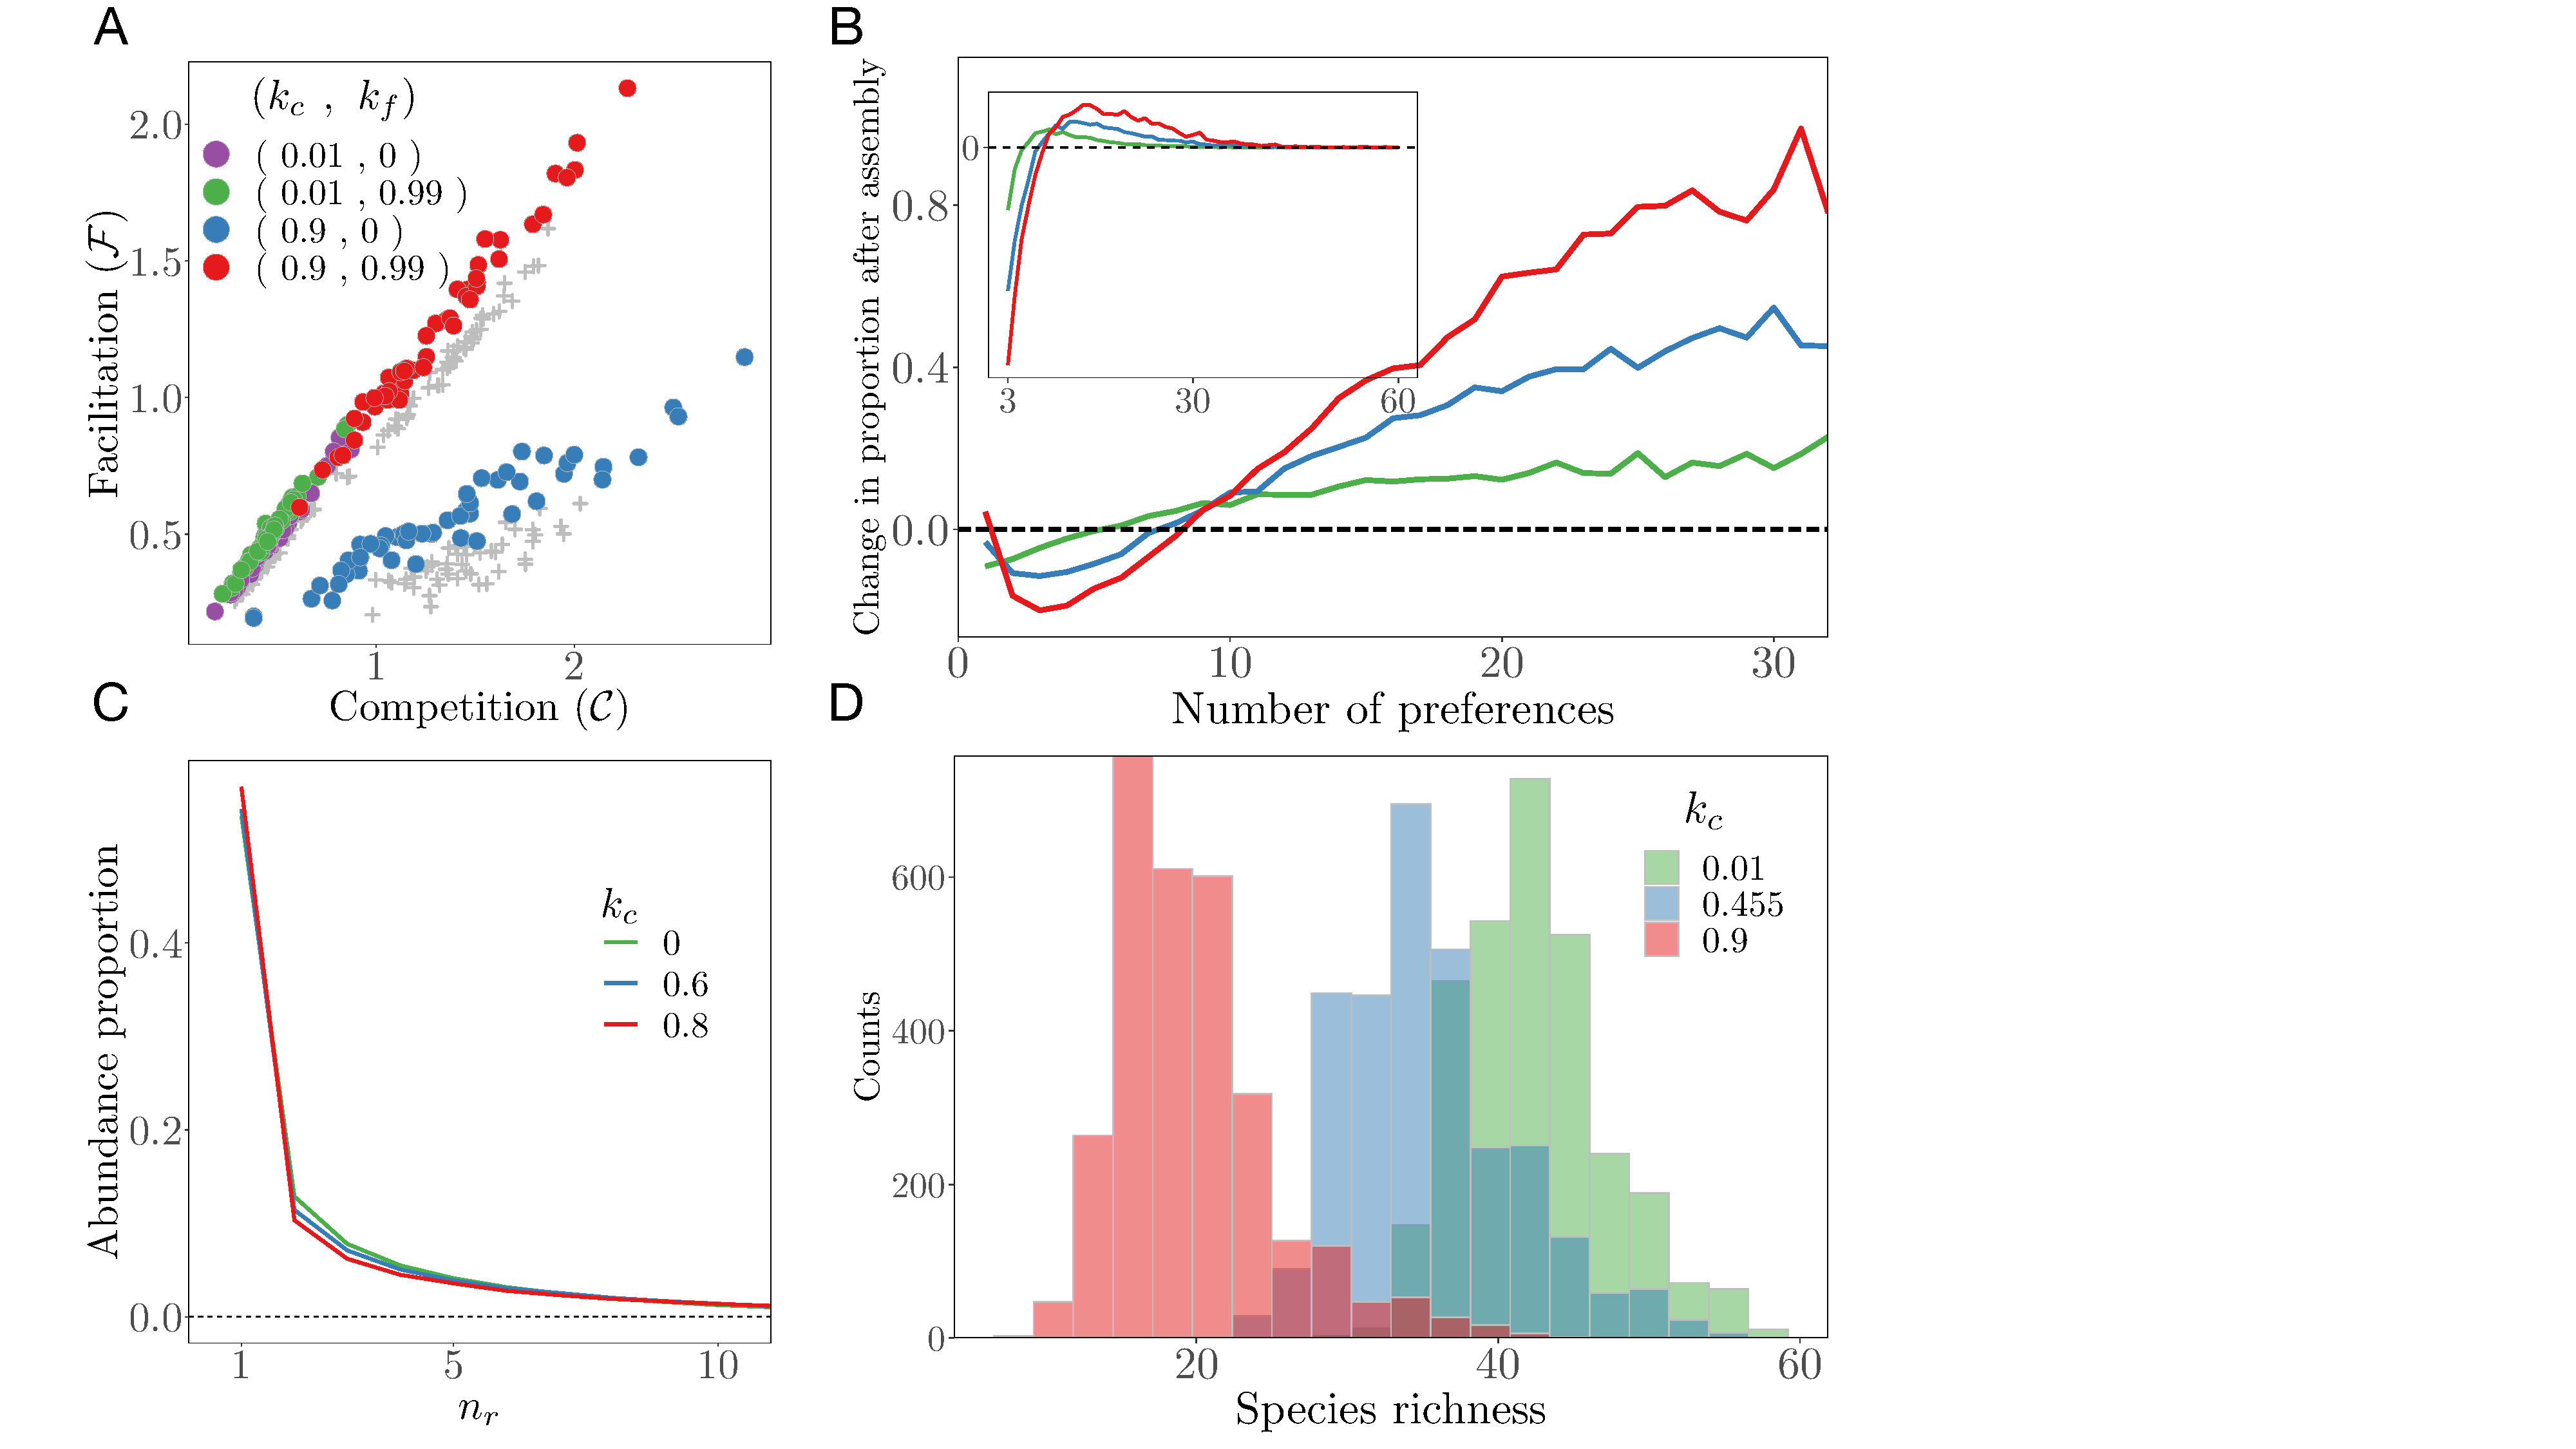
\includegraphics[width=1.1\columnwidth]{images/fig_assembly_results.pdf}
	\vspace{1pt}
	\caption{\textbf{Features of assembled parent communities}. \textbf{A}: Facilitation versus competition level in starting (grey dots) and assembled (coloured dots) communities for leakage $ l = 0.9 $ and different combinations of competition ($k_c$) and facilitation ($k_f$) factors. Communities assembled for each pair of $[k_c, k_f]$ values have the same colour. The assembled communities are always significantly more cooperative at the end of the assembly than at the start. \textbf{B}: Change in proportion of species in each n-preference consumer group ($\Delta n_r$, Methods; Step 2) before and after assembly, for different values of $k_c$ (legend in panel C) indicating that more generalist species are less prone to extinction during assembly. Values for $n_{r} > 30$ had too much uncertainty due to low sampling and therefore have been removed for clarity. \textbf{Inset:} $\Delta n_r$ is weighted by the abundance fraction  at equilibrium of each n-preference consumers group. \textbf{C}: Abundance fraction of the n-preference species groups for different values of $k_c$. \textbf{D}: Distributions of species richness values of parent communities assembled under different $k_c$ values. Increasing competitiveness tends to decrease species richness.}
	\label{fig:assembly}
\end{adjustwidth}
\end{figure}

\subsection*{Reducing competition increases coalescence success}

Figure \ref{fig:random_coalescence} shows that communities with lower net competition values tend to perform better in coalescence as seen by the positive relationship between parent community dominance ($S_{1,2}$) and the quantity ($\mathcal{C}_1 - \mathcal{F}_1) - (\mathcal{C}_2 - \mathcal{F}_2$)  (Fig~\ref{fig:random_coalescence}C). That is, communities that emerge following coalescence tend to have greater similarity with the less net competitive parent. This trend holds at higher values of leakage, where cooperation levels are significant (Fig~\ref{fig:random_coalescence}B), but with a clear critical point (the yellow line reverses in direction at a value of effective competition difference). This pattern is driven by the fact that less competitive parent communities deplete resources more efficiently and achieve a higher species richness (Fig~\ref{fig:random_coalescence}D; \nameref{S1_model}). All these results also qualitatively hold for microbial communities that have consumer guild structure (\nameref{S4_guilds}).

\begin{figure}[t]
\begin{adjustwidth}{-1.5in}{0in}
    \centering 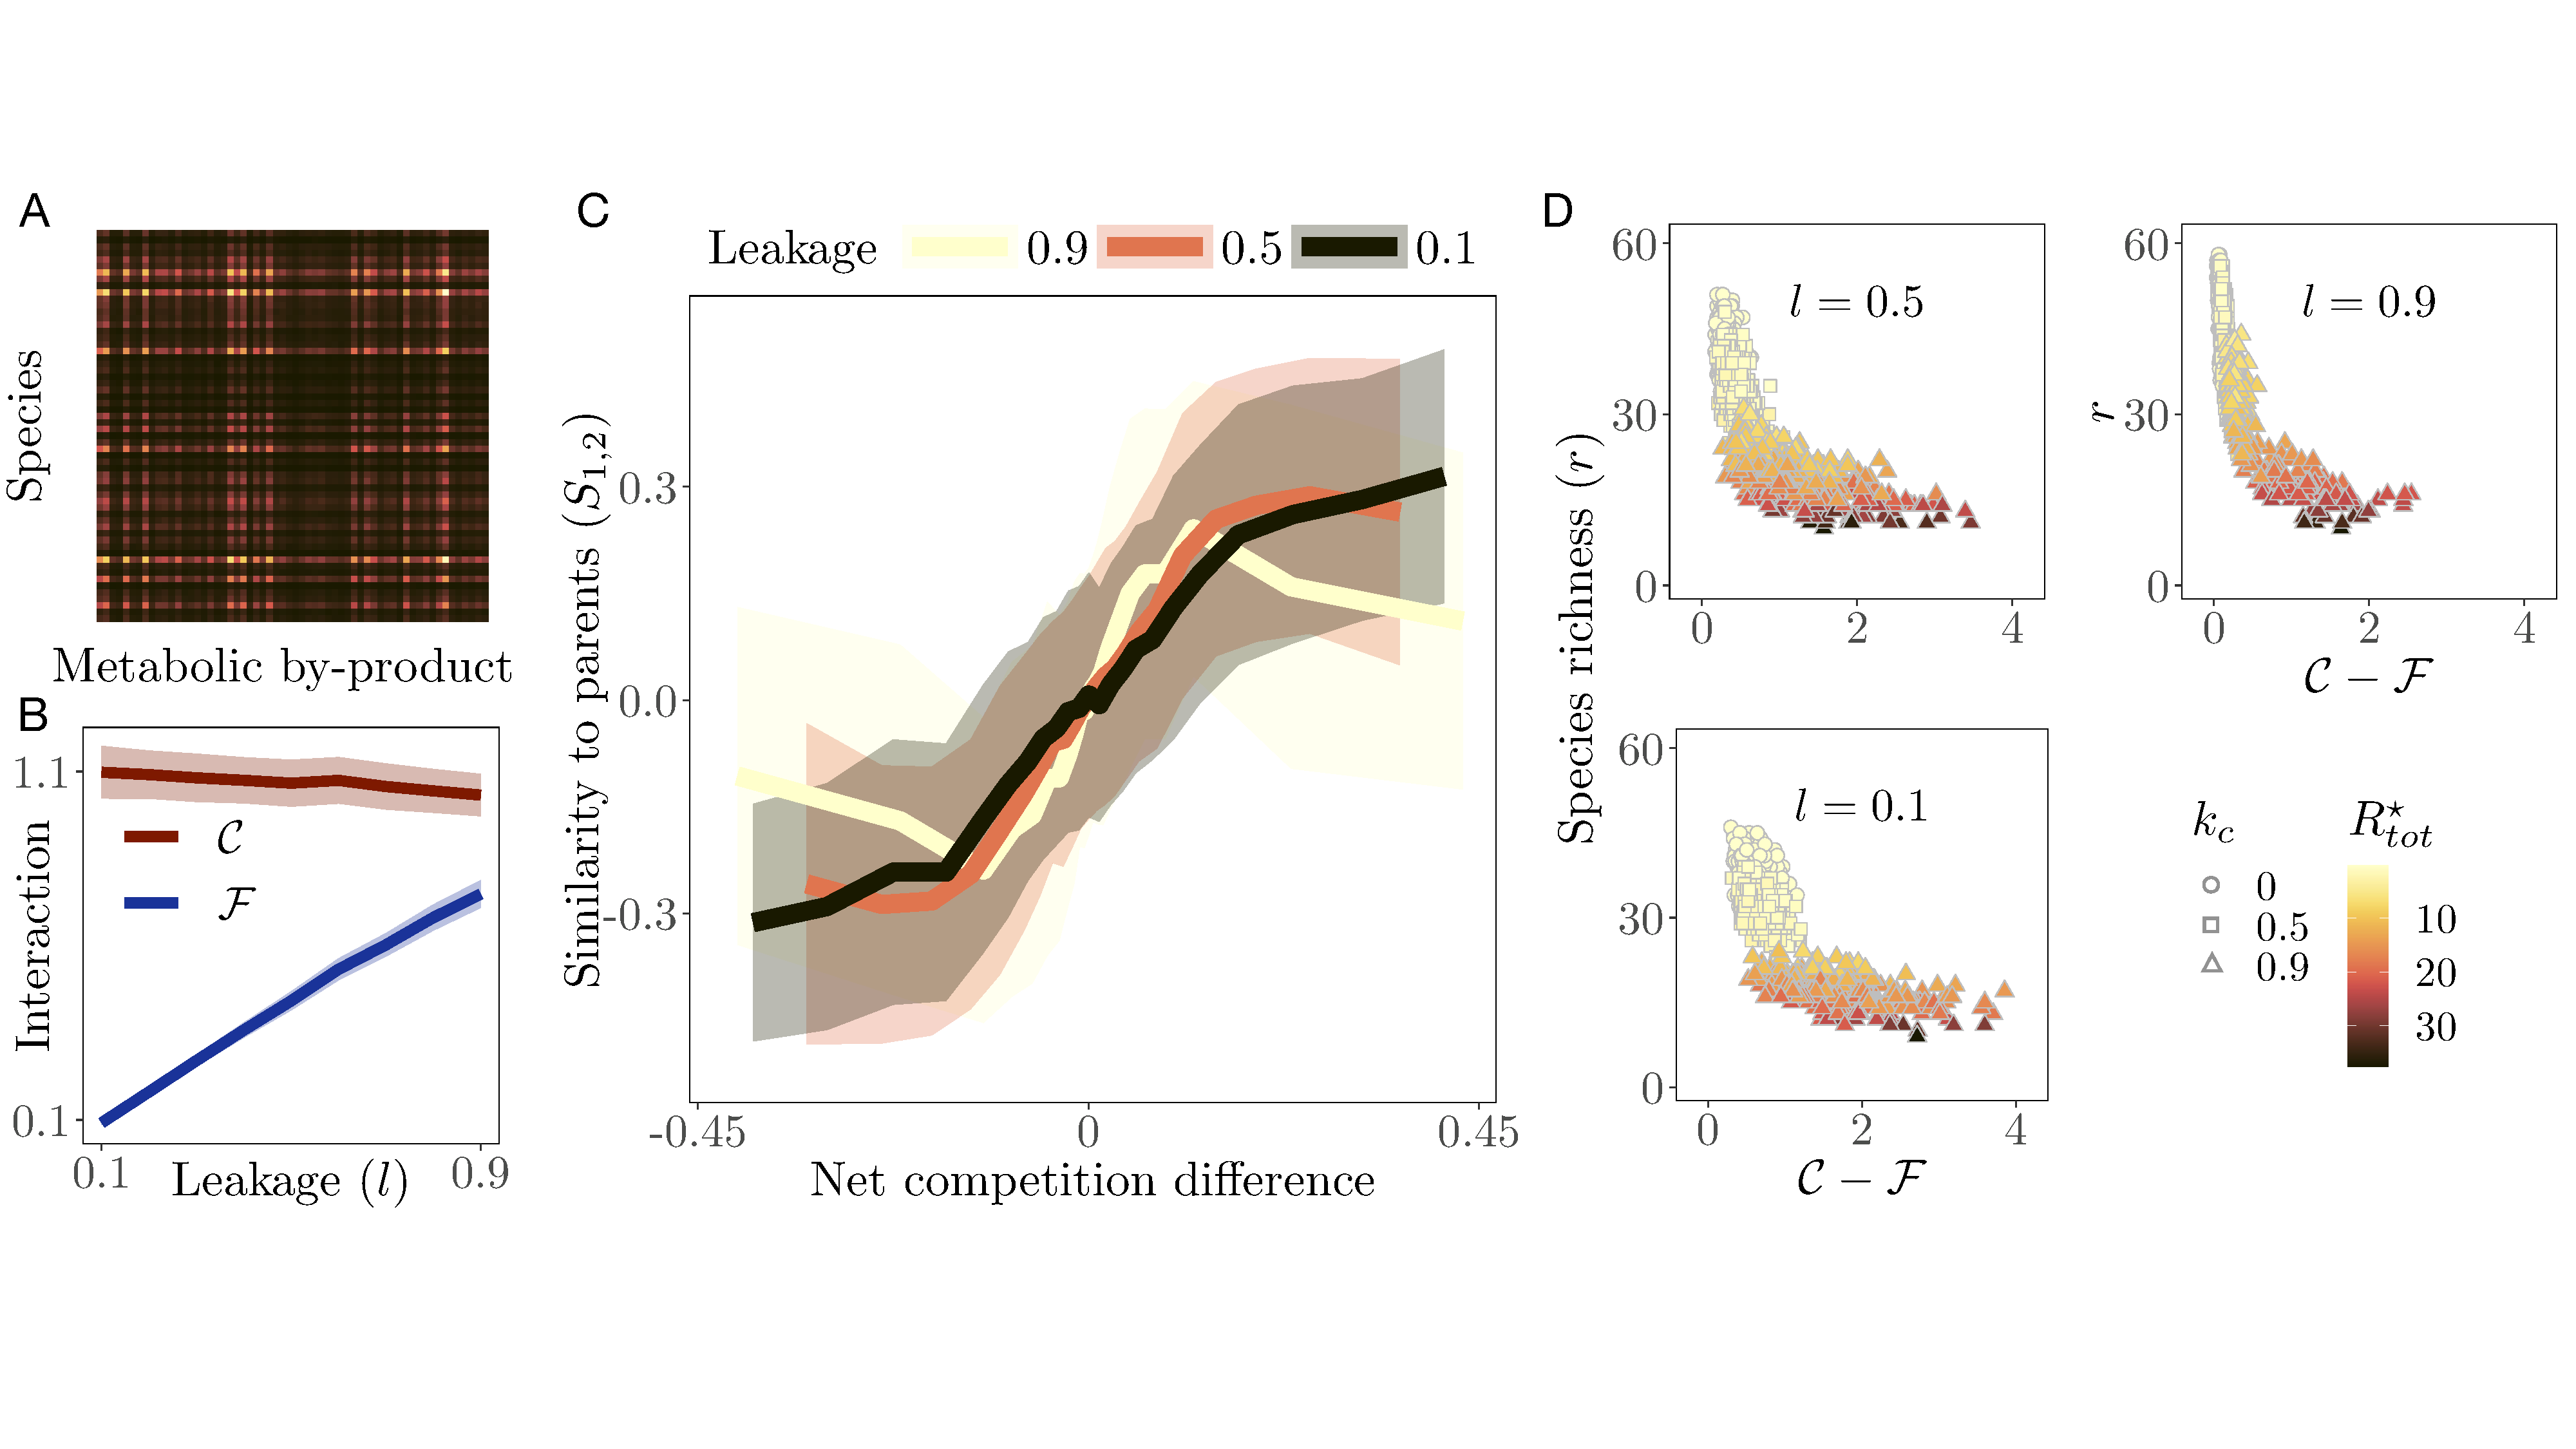
\includegraphics[width=1.3\columnwidth]{images/fig_random_coalescence.pdf}
    \vspace{1pt}
    \caption{\textbf{Community coalescence between pairs of randomly picked communities with same leakage.} {\bf A}: Example of the secretion matrix with elements $(C D)_{\alpha k}$ representing the total leakage of resource $k$ by species $\alpha$. {\bf B}: Community-level competition $\mathcal{C}$ (dark red) and facilitation $\mathcal{F}$ (blue) averaged across simulations for each leakage value. Since competition does not depend on the leakage, it remains consistently high throughout. Facilitation, on the other hand, increases linearly with leakage. {\bf C}: Parent community dominance $(S_{1, 2})$ as function of net competition difference ($\mathcal{C}_1 - \mathcal{F}_1) - (\mathcal{C}_2 - \mathcal{F}_2$) (solid lines $\pm$ 1 standard deviation (shaded)), binned (20 bins) over communities with similar x axis values, for three community-wide leakage levels. The post-coalescence community is more similar to its less (net) competitive parent. {\bf D}: Species richness $(r)$ as a function of net competition in parent communities, coloured by total resource concentration at steady state $(R_{tot}^{\star})$. The observed negative correlation for all values of leakage shows that communities with lower net competition tend to be more species-rich and also better at depleting resources (brighter coloured values, corresponding to lower levels of $R_{tot}^{\star}$ are scattered towards the top left of the plots).}
    \label{fig:random_coalescence}
\end{adjustwidth}
\end{figure}

\subsection*{Cooperation further enhances coalescence success}

Figure \ref{fig:recursive_coalescence} shows that when a community ($B$) whose leakage fraction increases successively during recursive coalescence events with another ($A$) with a fixed leakage level, the former becomes increasingly dominant. The result is consistent for a range of leakage values of community $A$. This shows that increasing cooperation levels enhance coalescence success.

\begin{figure}[t]
\begin{adjustwidth}{-1.5in}{0in}
    \centering 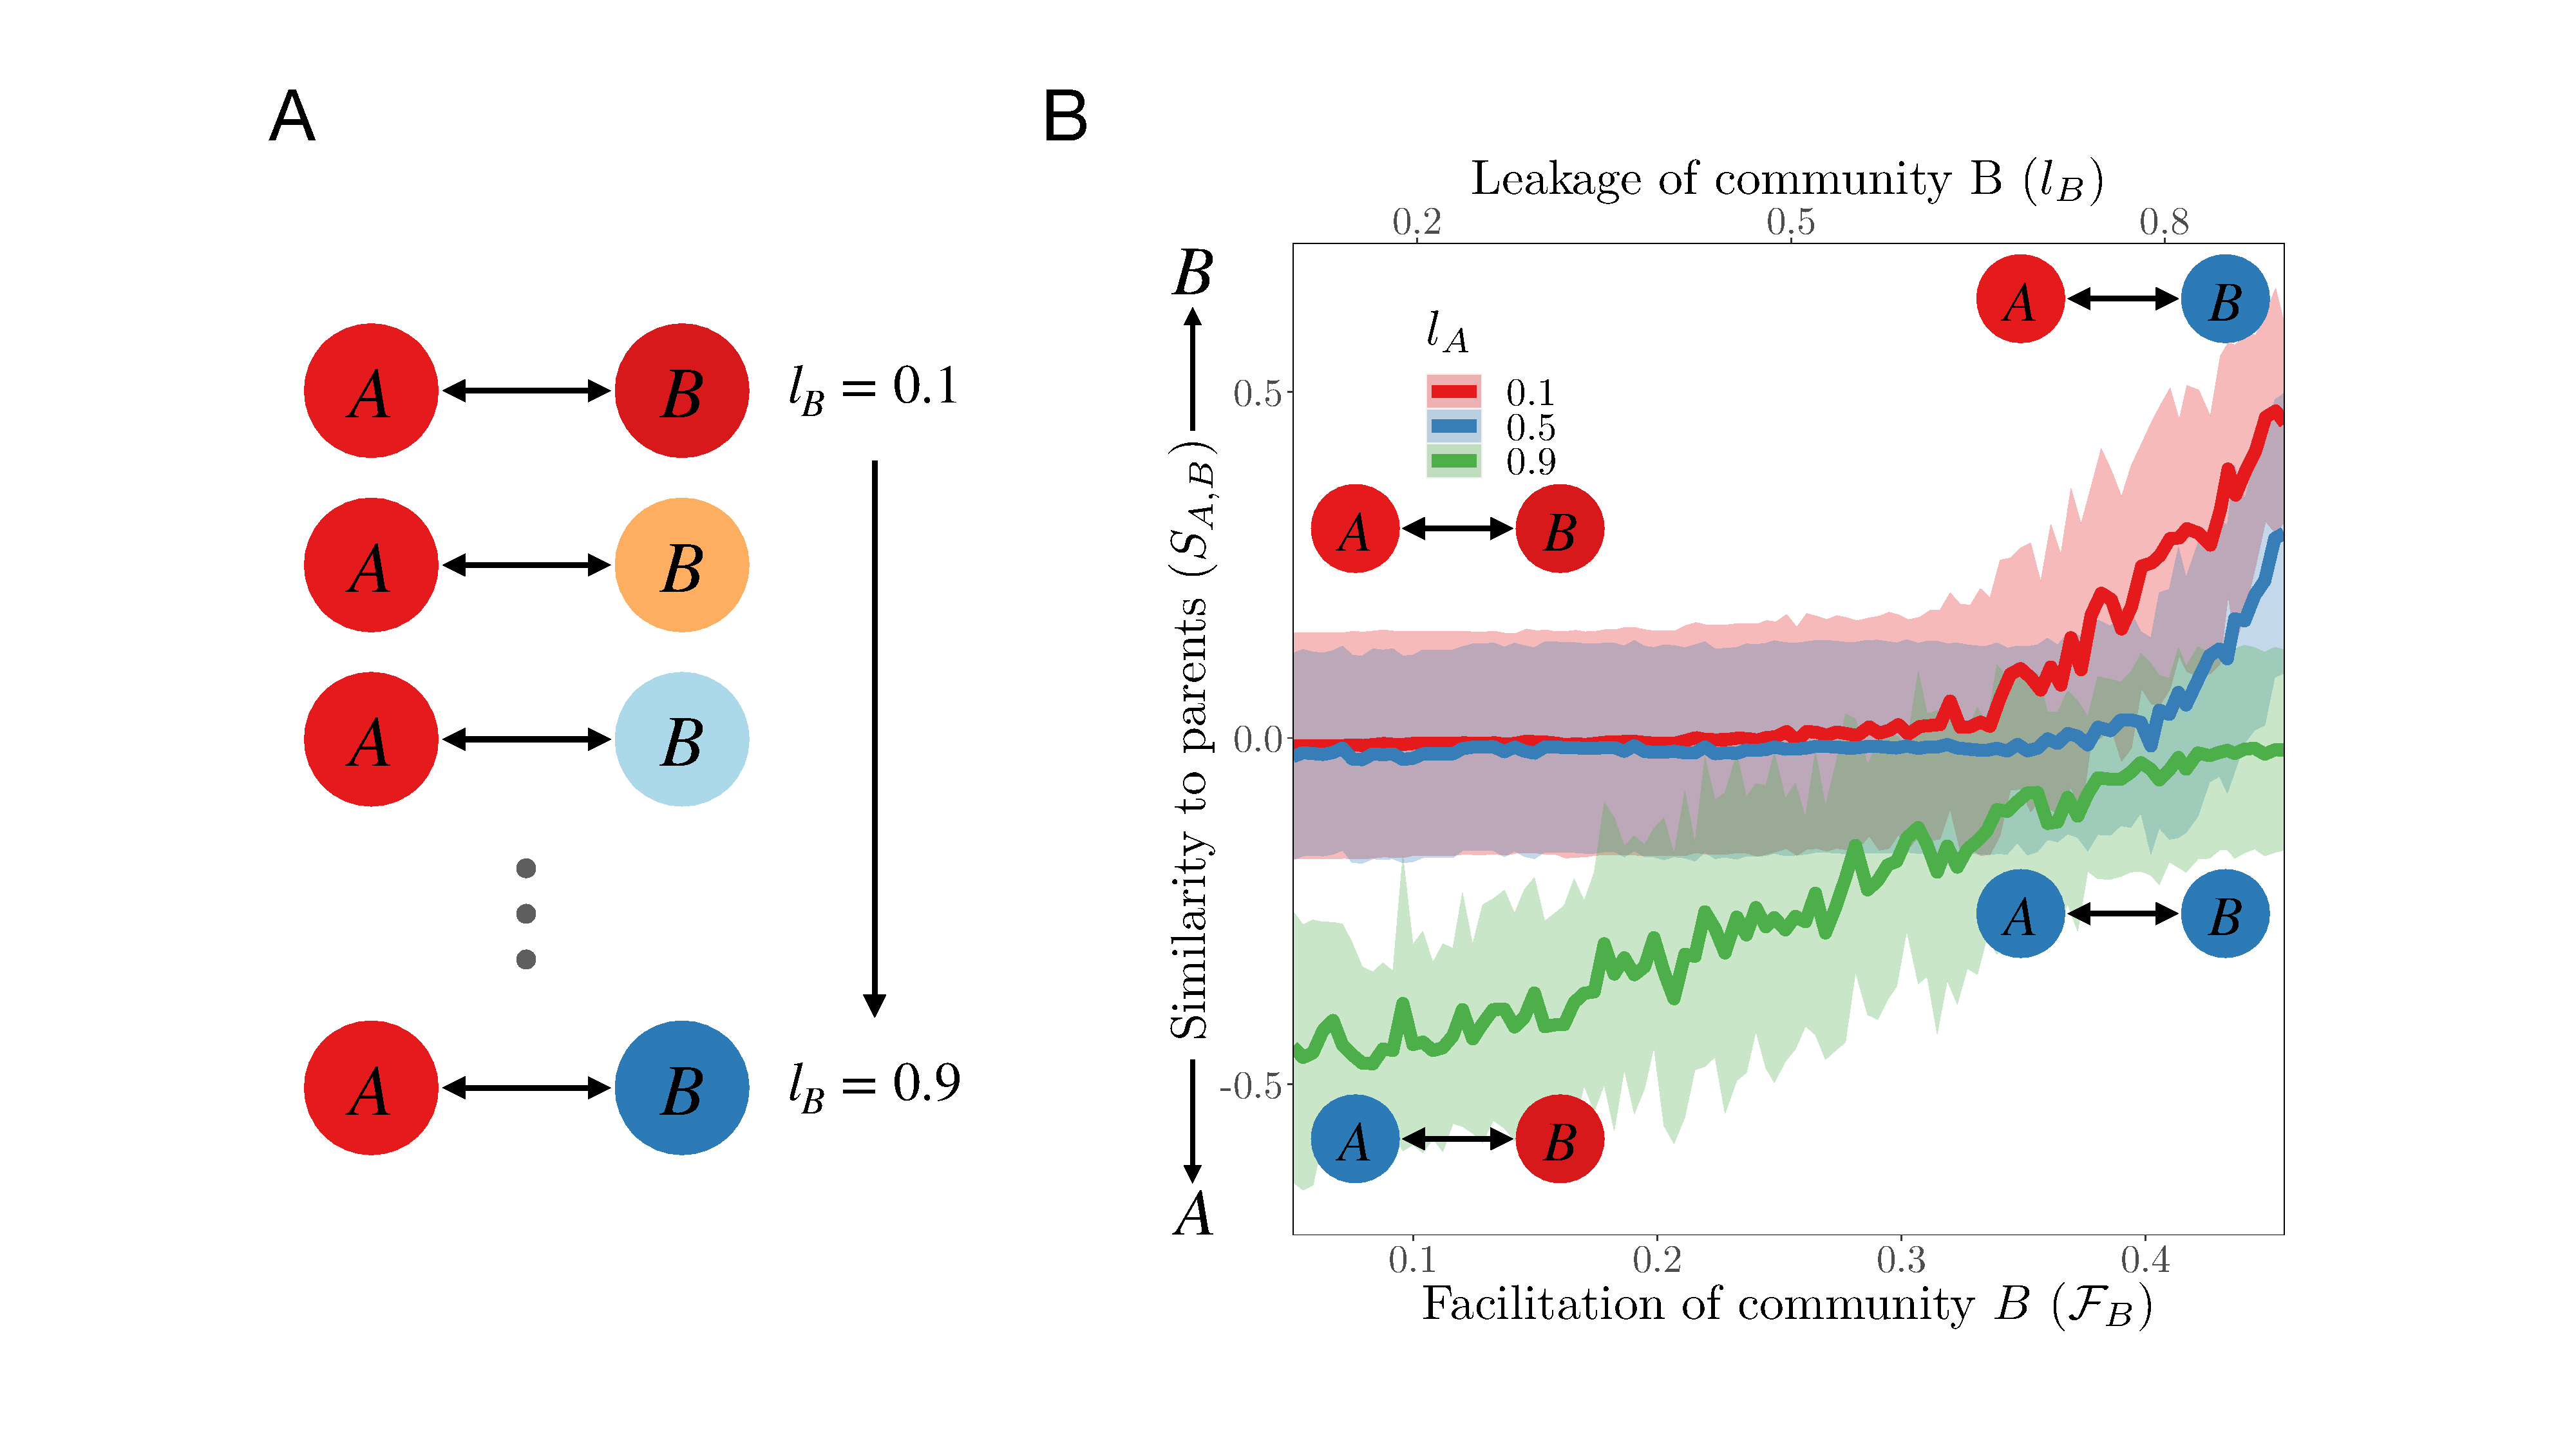
\includegraphics[width=1.3\columnwidth]{images/fig_recursive_coalescence.pdf}
    \vspace{1pt}
    \caption{\textbf{Recursive coalescence between microbial communities.} \textbf{A}: Sketch of the simulation set up. The same pair of communities $(A, B)$ is recursively coalesced, with the leakage of $B$ gradually increasing after each coalescence event for three levels of leakage of A, and 25 replicates per $l_A$ value. \textbf{B}: Parent community dominance after coalescence between communities $A$ and $B$, as a function of facilitation level of community $B$, $\mathcal{F}_B$ (bottom x axis), and leakage of community $B$, $l_B$ (top x axis). Each curve corresponds to a different value of $l_A$. Shaded regions are $\pm \sigma$. Dominance of parent community $B$ after coalescence increases with $l_B$, implying that higher cooperation levels enhance coalescence success.}
    \label{fig:recursive_coalescence}
\end{adjustwidth}
\end{figure}

\subsection*{Community evolution under repeated coalescence events}

Figure~\ref{fig:serial_coalescence} shows that on average, competition level significantly reduces and facilitation level increases during repeated coalescence events. Along with this, the average maintenance cost of species present in the resident community decreases with the number of coalescence exposures, and so does average resource abundance at equilibrium (Fig~\ref{fig:serial_coalescence}C and D), indicating that resource depletion ability improves in the process. In addition, the sub-population of resource specialists (that consume only one resource) increases with the number of coalescence events, while the rest of the species groups decrease in abundance (Fig~\ref{fig:serial_coalescence}E). Finally, the number of successful invasions into the resident community decreases function of number of coalescence events, while its species richness increases (Fig~\ref{fig:serial_coalescence}F). Taken together, these results show that communities composed of non-competing specialists that cooperate among themselves (Fig~\ref{fig:serial_coalescence}B and E) and reduce their respective metabolic costs (Fig~\ref{fig:serial_coalescence}C), improve their overall resource depletion ability (Fig~\ref{fig:serial_coalescence}D). This, in turn, makes them more resistant to multi-species invasions and therefore more successful in pairwise coalescence events (Fig~\ref{fig:serial_coalescence}F). 

\begin{figure}[ht!]
\begin{adjustwidth}{-1.5in}{0in}
    \centering
    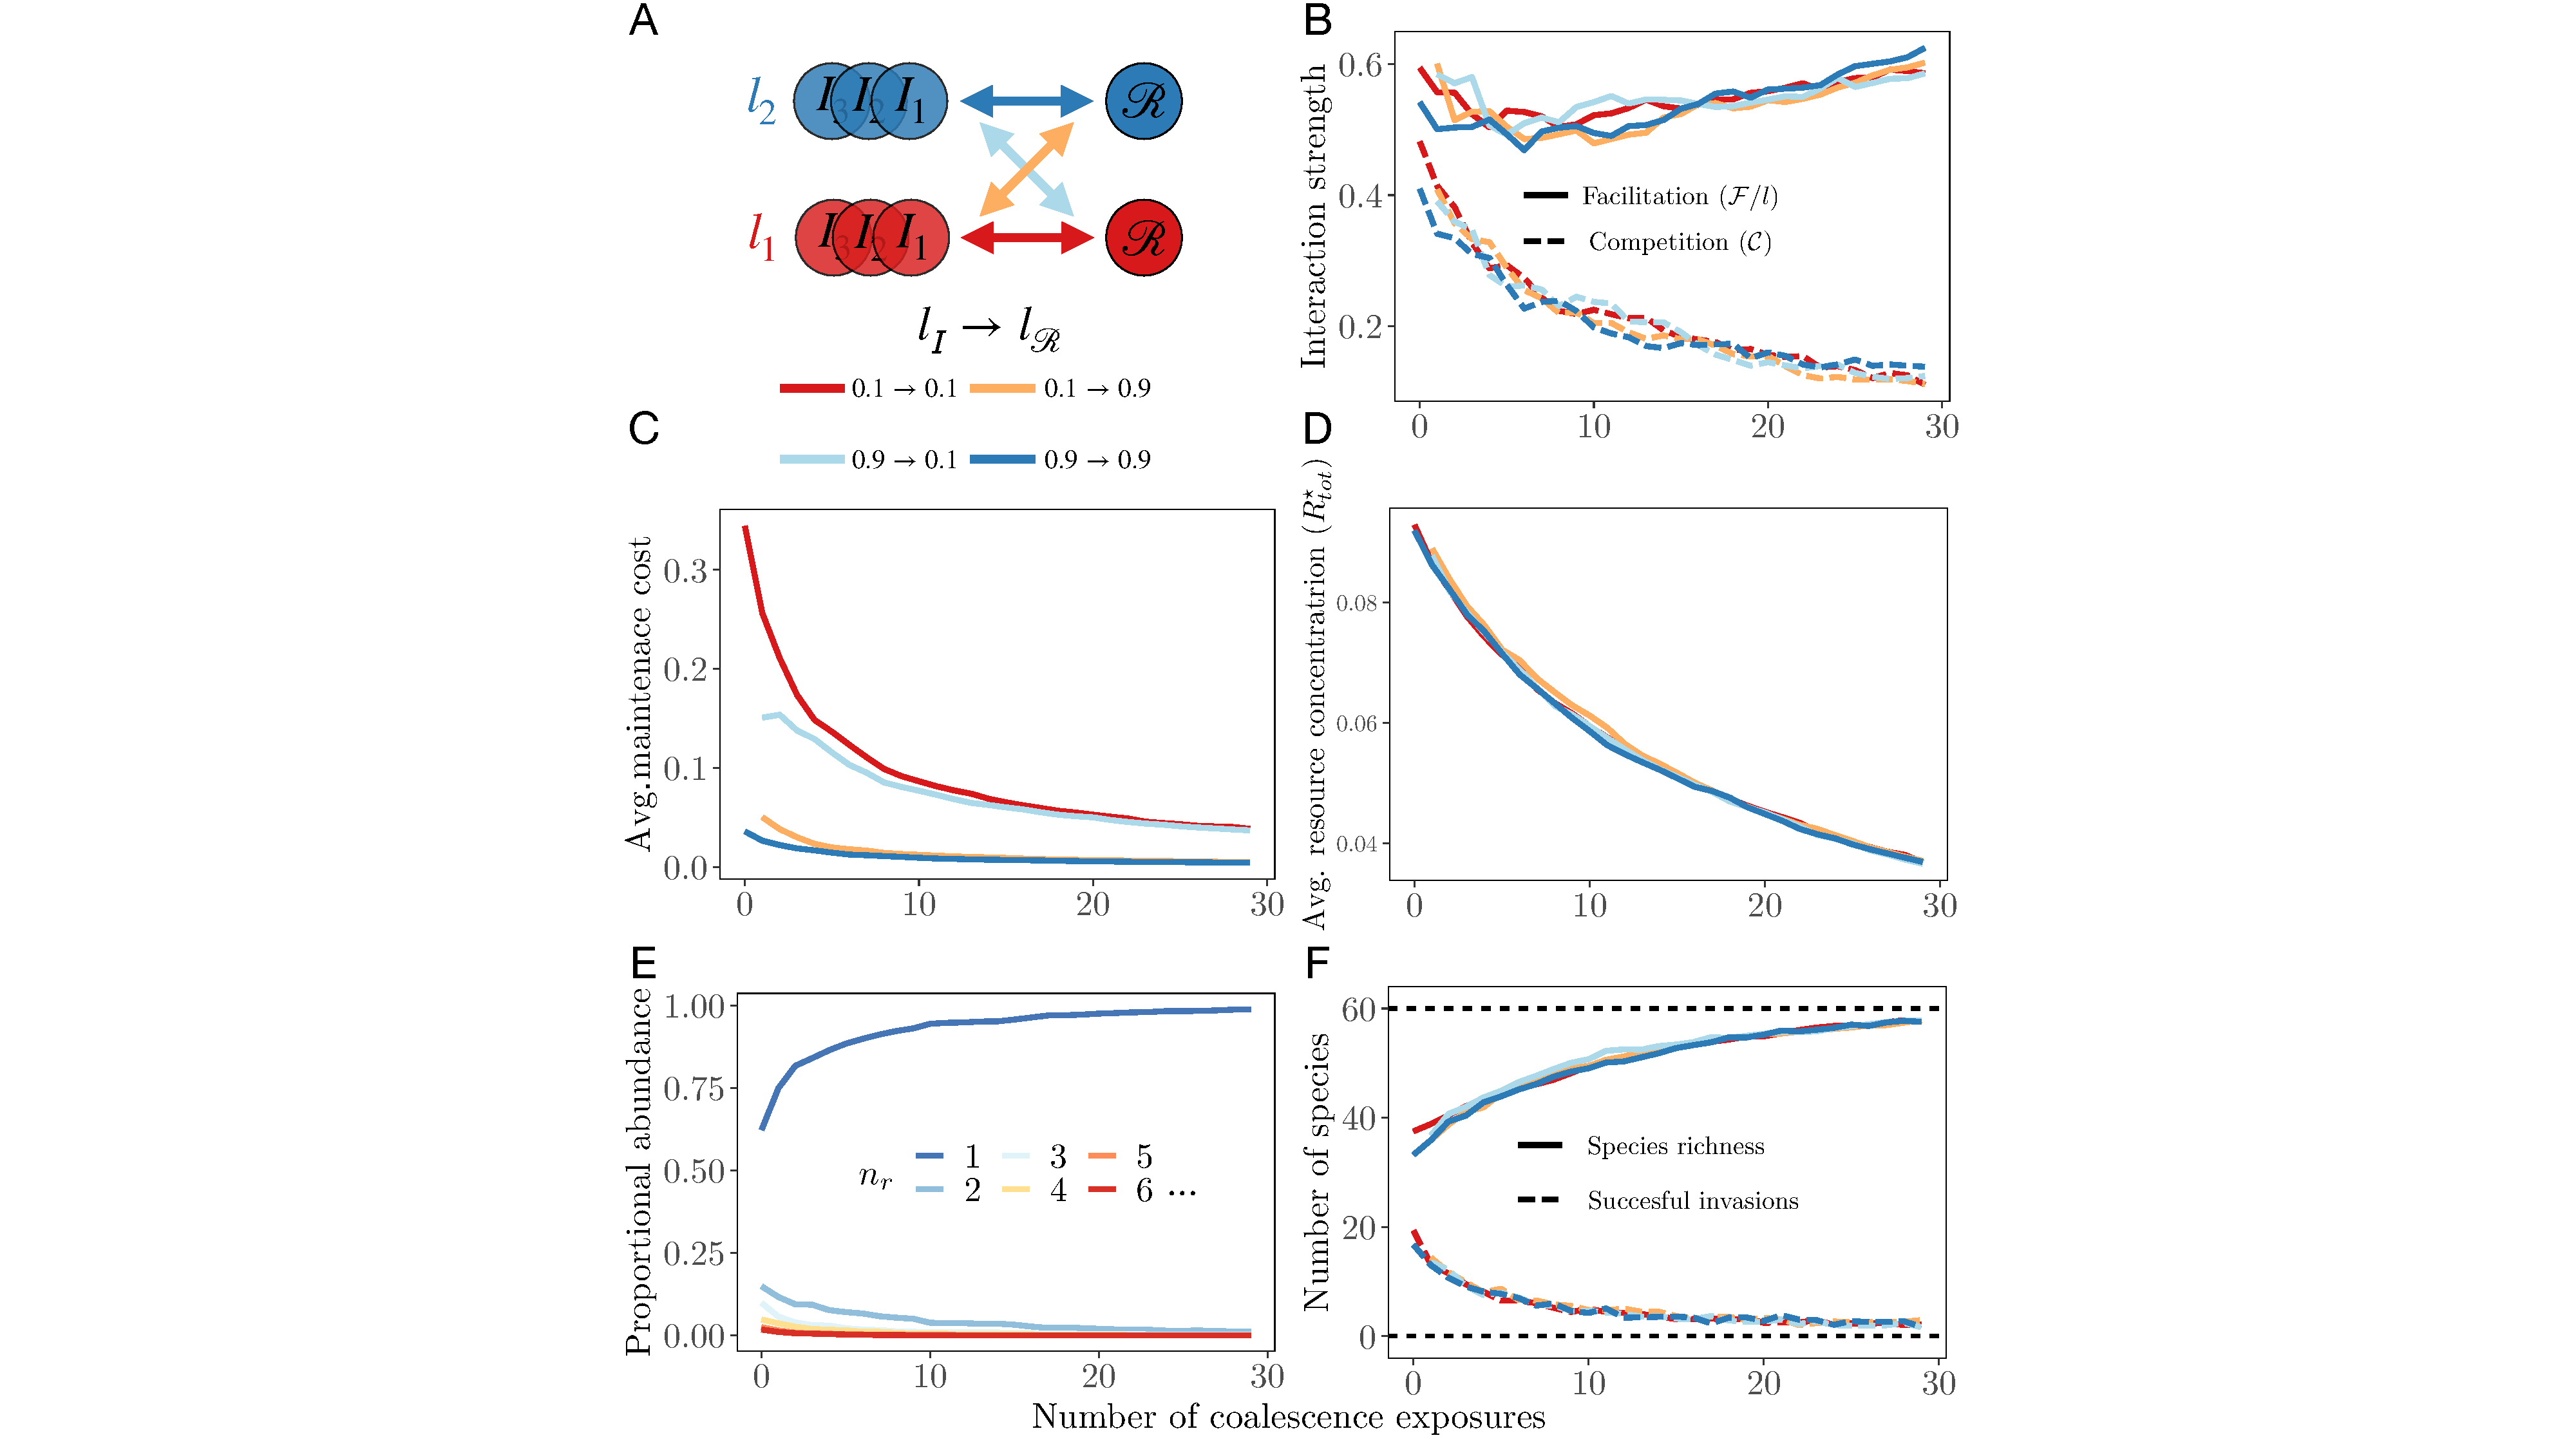
\includegraphics[width=1.15\columnwidth]{images/fig_serial_coalescence.pdf}
    \vspace{15pt}
    \caption{\textbf{Serial coalescence of microbial communities.} \textbf{A}: Sketch of the simulation set up. Resident communities ($\mathcal{R}$, upper circles) with leakage $l_{\mathcal{R}}$ are successively coalesced with randomly sampled invader communities ($\mathcal{I}$, lower circles) with leakage $l_{\mathcal{I}}$ for all possible combinations of leakage values (arrows) $\boldsymbol{l}_{\mathcal{I}} = \boldsymbol{l}_{\mathcal{R}} = [0.1, 0.9]$. For each serial coalescence sequence, we examine as a function of number of coalescence events, the following community properties of $\mathcal{R}$: (\textbf{B}) community-level competition ($\mathcal{C}$, dashed lines) and facilitation ($\mathcal{F}$, solid lines); (\textbf{C}) average species maintenance cost; (\textbf{D}) average resource concentration at equilibrium; (\textbf{E}) abundance fraction of each n-preference species group; and (\textbf{F}) number of successful invasions and with species richness. All the measures are averaged across 20 replicates. The standard deviation is decreasing along the x-axis and is never more than 40\% of the mean for all the curves (not shown to reduce clutter). Abundance fraction of species with $n_r > 5$ was negligible and is not plotted for clarity.}
    \label{fig:serial_coalescence}
\end{adjustwidth}
\end{figure}

\section*{Discussion}

Our findings offer new mechanistic insights in the dynamics and outcomes of microbial community coalescence by explicitly considering the balance between competition and cooperation; two key interactions of real microbial communities \cite{Machado2021, Pascual-Garcia2020}. Specifically, we find that communities harbouring less competing and more cooperative species (that is, having lesser net competition) dominate after coalescence because they are better at depleting resources and resisting invasions. Therefore, when a community undergoes a series of coalescence events, its competitiveness decreases and cooperativeness increases, along with its species richness, resource use efficiency, and resistance to invasions. These results provide a theoretical foundation for hypotheses suggested recently\cite{Castledine2020, Rillig2015}, and mechanistic insights into empirical studies that have demonstrated the importance of cross-feeding interactions on community coalescence \cite{Sierocinski2017}.

Our result based on coalescence between pairs of random communities at very low leakage (black line in Fig~\ref{fig:random_coalescence}C) essentially extends the results of \cite{Tikhonov2016} to communities with both competitive and cooperative interactions. Tikhonov showed that coalescence success is predicted by minimizing community-level competition through the optimisation of resource niche partitioning, which also guarantees maximization of resource depletion efficacy. Here we show that, similarly, the successful community is the one that achieves lower {\it net} competition ($\mathcal{C}-\mathcal{F}$), which also predicts community-level resource depletion efficacy as well as species richness (Fig~\ref{fig:random_coalescence}D). Thus, simultaneously reducing competition and increasing cooperation together drives the outcome of community coalescence. Therefore, the quantity $-(\mathcal{C}-\mathcal{F}) = \mathcal{F}-\mathcal{C}$ is also a measure of the ``cohesiveness'' of a microbial community. However, we also find that at extreme value of leakage ($l = 0.9$), there is a critical level of net competition difference beyond which coalescence success decreases again (yellow line in
Fig~\ref{fig:random_coalescence}C). This suggests that in the regime of high cooperation and competition, (high leakage, and tail ends of the curve) facilitative links in fact become detrimental. A similar result has been reported reported in \cite{Pascual-Garcia2017}. This critical value is not seen when the cost function does not include leakage (Fig. S2). Interestingly, we also find that this phenomenon is very weak when biologically-realistic guild structure is present (Fig. S6). These effects of extreme leakage (and facilitation) on coalescence success cannot be predicted by our model analyses (\nameref{S1_model}), and merit further investigation in future research, provided such high leakage levels are biologically feasible.

In our model systems, species compete not only for resources leaked by other species, but also for resources leaked by themselves, i.e., species may leak metabolic by-products that are also encoded in their consumer preferences vector. Leakage of metabolic resources is a pervasive phenomenon in the microbial world \cite{Morris2015, Kallus2017}, and has been shown to exist also in resources necessary for growth, even in situations when those essential metabolites are scarce \cite{Paczia2012, Silva2015}. Although it may seem counter-intuitive for microbes to secrete metabolites essential for their own growth, such leakage can be advantageous, especially in bacteria, as ``flux control'' or growth-dilution mechanisms which provide short-term growth benefits in crowded environments \cite{Yamagishi2020,Yamagishi2021}.

Our recursive coalescence simulations (Fig~\ref{fig:recursive_coalescence}A) allowed us to establish that coalescence success is enhanced by cooperative interactions. This result is consistent with past theoretical work showing that mutualistic interactions are expected to increase structural stability by decreasing effective competition \cite{Bastolla2009}. It is also consistent with recent theoretical results on single species invasions in microbial communities  \cite{Kurkjian2021}. Nonetheless, this finding hinges on our choice of the cost function (Eq~\eqref{eq:cost}; \nameref{S1_model}). This cost function, which was motivated by biological considerations, imposed an efficiency cost to species with lower leakage, ensuring that all consumers, independently of their leakage fraction, depleted resources to the same concentration on average (see \nameref{S1_model}). This allowed us to perform coalescence events between communities harbouring species with different leakage without introducing a bias towards the more efficient species. This choice corresponds biologically to the interpretation of leakage as an efficiency factor in the conversion from energy to biomass (Eq~S2 in Supplementary information). As a consequence, higher leakage species reach, in general, lower abundances at equilibrium \cite{Wieser1994}.

Our findings about the evolution of community-level properties in response to repeated community-community encounters (Fig~\ref{fig:serial_coalescence}) suggest that it might be possible to identify functional groups of microbes or microbial traits that are are a ``smoking gun'' of past coalescence events experienced by a given community \cite{Rillig2015}. Additionally, our finding that members of communities with a history of coalescence are likely to be become increasingly resistant to further community invasions suggests a novel and potentially economical way to assemble robust microbial communities. We also found that repeated coalescence events contributed to increase species richness, offering another mechanism that may help explain differences in microbial diversity across locations and environments \cite{Rillig2015}. 

Our finding that resident communities exposed to repeated community invasions were mainly composed of cooperative specialists (Fig~\ref{fig:serial_coalescence}B and E) is due to our assumption that all resources were supplied, and at a fixed rate. This allowed  specialists to survive because their only source of energy was always provided. This property may not be as commonly seen in real communities, where fluctuations in resource supply are common. Ignoring environmental fluctuations allowed us to focus on coalescence outcomes in terms of the species interaction structure alone. While this assumption may be sensible in some cases \cite{Acosta2015}, it is an oversimplification in others \cite{Albright2020}. Therefore, studying the complex interplay between biotic interactions and environmental factors, e.g., by allowing substrate diversification from a single supplied resource \cite{Goldford2018, Marsland2019}, or perturbing the supply vector periodically to simulate some form of seasonality, is a promising direction for future research. In such cases, we expect a more balanced mix of generalists and specialists, such that only the competitive interactions necessary to diversify the available carbon sources will persist upon coalescence events, but above that threshold, the results presented here (Figs~\ref{fig:random_coalescence}, \ref{fig:recursive_coalescence}, and \ref{fig:serial_coalescence}) would be recovered. 

Assuming a core leakage and metabolism common to the whole community, made the assembly dynamics computationally tractable, while ensuring that the system was not far away from the conditions of real communities \cite{Marsland2019, Marsland2020}. The assumption of common leakage was relaxed in the recursive coalescence procedure. In addition, both the community-wide fixed leakage and core metabolism assumptions were relaxed in the serial coalescence simulations, thus using the model in its fully general form as seen in Eqs~\ref{eq:Model}. Finally, to retain an analytically tractable theoretical setting for an otherwise complex system, we assumed binary consumer preferences, linear consumer functional responses, and resources of equal energetic value throughout. While this is a promising avenue for future work, we expect our results to be qualitatively robust to relaxation of these constraints, based on recent work on microbial community assembly dynamics using the same general model \cite{Marsland2019, Marsland2020}.

Encounters between microbial communities are becoming increasingly frequent \cite{Seebens2017}, and mixing of whole microbial communities is gaining popularity for bio-engineering \cite{Rillig2016}, soil restoration \cite{Calderon2017}, faecal microbiota transplantation \cite{Wang2019, Wilson2019}, and the use of probiotics \cite{Lindemann2016}. We present a framework which relates the structure of species interactions in microbial communities to the outcome of community coalescence events. Although more work is required to bridge the gap between theory and empirical observations, this study constitutes a key step in that direction.

\section*{Supporting information}

% CITE SI USING (For more information, see \nameref{S1_Appendix}.)

% Include only the SI item label in the paragraph heading. Use the \nameref{label} command to cite SI items in the text.
\paragraph*{Supporting text section 1}\textbf{--  Further details of the mathematical model.}
\label{S1_model}
\paragraph*{Supporting text section 2}\textbf{--  Modulating net competition levels.}
\label{S2_modulating}
\paragraph*{Supporting text section 3}\textbf{--  Further details of the community coalescence simulations.}
\label{S3_simulation_details}
\paragraph*{Supporting text section 4}\textbf{--  Adding consumer guild structure.}
\label{S4_guilds}

\paragraph*{Fig S1} Consequence of relaxing the assumption of leakage dependence.
\label{S1Fig}
\paragraph*{Fig S2} Results  of  random  coalescence  procedure  without  imposing  the  efficiency cost (leakage dependence).
\label{S2Fig}
\paragraph*{Fig S3} Eigenvalues of J when evaluated
at equilibrium for two example communities.
\label{fig:S3Fig}
\paragraph*{Fig S4} Examples of differently-structured preference ($C$) and metabolic ($D$) matrices.
\label{fig:S4Fig}
\paragraph*{Fig S5} Auto-correlation of vector of species abundances in community B for consecutive re-assemblies of this community, along the studied leakage range.
\label{fig:S5Fig}
\paragraph*{Fig S6} Community coalescence with consumer guilds present.
\label{S6Fig}

\section*{Author Contributions}
\textbf{Conceptualization:} Pablo Lechón, Tom Clegg, Jacob Cook, Thomas P. Smith, Samraat Pawar\\[10pt]
\hspace{-14pt}\textbf{Methodology:} Pablo Lechón \\[10pt]
\hspace{-14pt}\textbf{Software and Visualizations:} Pablo Lechón \\[10pt]
\hspace{-14pt}\textbf{Writing – Original Draft Preparation:} Pablo Lechón \\[10pt]
\hspace{-14pt}\textbf{Writing – Review \& Editing:} Pablo Lechón, Tom Clegg, Jacob Cook, Thomas P. Smith, Samraat Pawar. \\[10pt]
\hspace{-14pt}\textbf{Funding Acquisition:} Samraat Pawar \\[10pt]

%\section*{Acknowledgments}
%THANK PEOPLE
\newpage 

\nolinenumbers

\begin{thebibliography}{10}

\bibitem{Fierer2006}
Fierer N, Jackson RB.
\newblock {The diversity and biogeography of soil bacterial communities}.
\newblock Proceedings of the National Academy of Sciences of the United States
  of America. 2006;103(3):626--631.
\newblock doi:{10.1073/pnas.0507535103}.

\bibitem{Huttenhower2012}
Huttenhower C, Gevers D, Knight R, Al E.
\newblock {Structure, function and diversity of the healthy human microbiome}.
\newblock Nature. 2012;486(7402):207–214.
\newblock doi:{10.1038/nature11234}.

\bibitem{McFall-Ngai2013}
McFall-Ngai M, Hadfield MG, Bosch TCG, Carey HV, Domazet-Lo{\v{s}}o T, Douglas
  AE, et~al.
\newblock {Animals in a bacterial world, a new imperative for the life sciences}.
\newblock Proceedings of the National Academy of Sciences of the United States of America. 2013;110(9):3229--3236.
\newblock doi:{10.1073/pnas.1218525110}.

\bibitem{Falkowski2008}
Falkowski PG, Fenchel T, Delong EF.
\newblock {The microbial engines that drive earth's biogeochemical cycles}.
\newblock Science. 2008;320(5879):1034--1039.
\newblock doi:{10.1126/science.1153213}.

\bibitem{Gilbert2014}
Gilbert JA, Jansson JK, Knight R.
\newblock {The Earth Microbiome project: Successes and aspirations}.
\newblock BMC Biology. 2014;12(69):12915--014.
\newblock doi:{10.1186/s12915-014-0069-1}.

\bibitem{Marsland2019}
Marsland R, Cui W, Goldford J, Sanchez A, Korolev K, Mehta P.
\newblock {Available energy fluxes drive a transition in the diversity, stability, and functional structure of microbial communities}.
\newblock PLoS Computational Biology. 2019;15(2):e1006793. doi:
  10.1371/journal.pcbi.1006793.
\newblock doi:{10.1371/journal.pcbi.1006793}.

\bibitem{Goldford2018}
Goldford JE, Lu N, Baji{\'{c}} D, Estrela S, Tikhonov M, Sanchez-Gorostiaga A,
  et~al.
\newblock {Emergent simplicity in microbial community assembly}.
\newblock Science. 2018;361(6401):469--474.
\newblock doi:{10.1126/science.aat1168}.

\bibitem{Goyal2018}
Goyal A, Maslov S.
\newblock {Diversity, Stability, and Reproducibility in Stochastically
  Assembled Microbial Ecosystems}.
\newblock Physical Review Letters. 2018;120(15):158102.
\newblock doi:{10.1103/PhysRevLett.120.158102}.

\bibitem{Friedman2017}
Friedman J, Higgins LM, Gore J.
\newblock {Community structure follows simple assembly rules in microbial
  microcosms}.
\newblock Nature Ecology and Evolution. 2017;1(5):41559--017.
\newblock doi:{10.1038/s41559-017-0109}.

\bibitem{Costello2012}
Costello EK, Stagaman K, Dethlefsen L, Bohannan BJM, Relman DA.
\newblock {The application of ecological theory toward an understanding of the
  human microbiome}.
\newblock Science. 2012;336(6086):1255--1262.
\newblock doi:{10.1126/science.1224203}.

\bibitem{Vila2019}
Vila JCC, Jones ML, Patel M, Bell T, Rosindell J.
\newblock {Uncovering the rules of microbial community invasions}.
\newblock Nature Ecology and Evolution. 2019;3(8):1162--1171.
\newblock doi:{10.1038/s41559-019-0952-9}.

\bibitem{Estrela2020}
Estrela S, Vila JCC, Lu N, Bajic D, Rebolleda-Gomez M, Chang CY, et~al.
\newblock {Metabolic rules of microbial community assembly}.
\newblock bioRxiv. 2020.
\newblock doi:{10.1101/2020.03.09.984278}.

\bibitem{Coyte2021}
Coyte KZ, Rao C, Rakoff-nahoum S, Foster KR.
\newblock {Ecological rules for the assembly of microbiome communities}.
\newblock PLOS Biol. 2021;19(2):e3001116.
\newblock doi:{10.1371/journal.pbio.3001116}.

\bibitem{Luo2020}
Luo X, Xiang X, Yang Y, Huang G, Fu K, Che R, et~al.
\newblock {Seasonal effects of river flow on microbial community coalescence
  and diversity in a riverine network}.
\newblock FEMS Microbiology Ecology. 2020;96(8).
\newblock doi:{10.1093/femsec/fiaa132}.

\bibitem{Vass2021}
Vass M, Sz{\'{e}}kely AJ, Lindstr{\"{o}}m ES, Osman OA, Langenheder S.
\newblock {Warming mediates the resistance of aquatic bacteria to invasion
  during community coalescence}.
\newblock Molecular Ecology. 2021;doi:{10.1111/mec.15800}.

\bibitem{Kort2014}
Kort R, Caspers M, van~de Graaf A, van Egmond W, Keijser B, Roeselers G.
\newblock {Shaping the oral microbiota through intimate kissing}.
\newblock Microbiome. 2014;2(1):1--8.
\newblock doi:{10.1186/2049-2618-2-41}.

\bibitem{Evans2020}
Evans SE, Bell-Dereske LP, Dougherty KM, Kittredge HA.
\newblock {Dispersal alters soil microbial community response to drought}.
\newblock Environmental Microbiology. 2020;22(3):905--916.
\newblock doi:{10.1111/1462-2920.14707}.

\bibitem{Rillig2015}
Rillig MC, Antonovics J, Caruso T, Lehmann A, Powell JR, Veresoglou SD, et~al.
\newblock {Interchange of entire communities: Microbial community coalescence}.
\newblock Trends in Ecology and Evolution. 2015;30(8):470--476.
\newblock doi:{10.1016/j.tree.2015.06.004}.

\bibitem{Rillig2016a}
Rillig M, Tsang A, Roy J.
\newblock {Microbial community coalescence for microbiome engineering}.
\newblock Front. Microbiol. 2016;7:1967
\newblock doi: {10.3389/fmicb.2016.01967}.

\bibitem{Rillig2016b}
Rillig MC, Lehmann A, Aguilar-Trigueros CA.
\newblock {Soil microbes and community coalescence}.
\newblock Pedobiologia. 2016;59(1-2):37--40.
\newblock doi:{10.1016/j.pedobi.2016.01.001}.

\bibitem{Castledine2020}
Castledine M, Sierocinski P, Padfield D, Buckling A.
\newblock {Community coalescence: An eco-evolutionary perspective}.
\newblock Philosophical transactions of the Royal Society of London Series B, Biological sciences. 2020;375(1798):20190252.
\newblock doi:{10.1098/rstb.2019.0252}.

\bibitem{Sierocinski2017}
Sierocinski P, Milferstedt K, Bayer F, Gro{\ss}kopf T, Alston M, Bastkowski S, et~al.
\newblock {A single community dominates structure and function of a mixture of multiple methanogenic communities}.
\newblock Current Biology. 2017;27(21):3390--3395.
\newblock doi:{10.1016/j.cub.2017.09.056}.

\bibitem{Gilpin1994}
Gilpin M.
\newblock {Community-level competition: Asymmetrical dominance}.
\newblock Proceedings of the National Academy of Sciences of the United States of America. 1994;91(8):3252--3254.
\newblock doi:{10.1073/pnas.91.8.3252}.

\bibitem{Toquenaga1997}
Toquenaga Y.
\newblock {Historicity of a simple competition model}.
\newblock Journal of Theoretical Biology. 1997;187(2):175--181.
\newblock doi:{10.1006/jtbi.1997.0428}.

\bibitem{Tikhonov2016}
Tikhonov M.
\newblock {Community-level cohesion without cooperation}.
\newblock eLife. 2016;5:e15747. doi: 10.7554/eLife.15747.
\newblock doi:{10.7554/eLife.15747}.

\bibitem{Pascual-Garcia2020}
Pascual-Garc{\'{i}}a A, Bonhoeffer S, Bell T.
\newblock {Metabolically cohesive microbial consortia and ecosystem functioning}.
\newblock Philosophical Transactions of the Royal Society B: Biological Sciences. 2020;375(1798):0190245.
\newblock doi:{10.1098/rstb.2019.0245}.

\bibitem{Marsland2020}
Marsland, R., Cui, W. and Mehta, P.
\newblock {A minimal model for microbial biodiversity can reproduce experimentally observed ecological patterns.}.
\newblock Sci Rep. 2020;10, 3308. 
\newblock doi:{doi.org/10.1038/s41598-020-60130-2}.

\bibitem{Lu2018}
Lu N, Sanchez-gorostiaga A, Tikhonov M, Sanchez A.
\newblock {Cohesiveness in microbial community coalescence}.
\newblock bioRxiv. 2018; p. 282723
\newblock doi:{10.1101/282723}.

\bibitem{Hansen2007}
Hansen SK, Rainey PB, Haagensen JAJ, Molin S.
\newblock {Evolution of species interactions in a biofilm community}.
\newblock Nature. 2007;445(7127):533–536.
\newblock doi:{10.1038/nature05514}.

\bibitem{Lawrence2012}
Lawrence D, Fiegna F, Behrends V, Bundy JG, Phillimore AB, Bell T, et~al.
\newblock {Species interactions alter evolutionary responses to a novel
  environment}.
\newblock PLoS Biology. 2012;10(5):e1001330. doi: 10.1371/journal.pbio.1001330.
\newblock doi:{10.1371/journal.pbio.1001330}.

\bibitem{Embree2015}
Embree M, Liu JK, Al-Bassam MM, Zengler K.
\newblock {Networks of energetic and metabolic interactions define dynamics in microbial communities}.
\newblock Proceedings of the National Academy of Sciences of the United States of America. 2015;112(50):15450–15455.
\newblock doi:{10.1073/pnas.1506034112}.

\bibitem{Rivett2018}
Rivett DW, Jones ML, Ramoneda J, Mombrikotb SB, Ransome E, Bell T.
\newblock {Elevated success of multispecies bacterial invasions impacts community composition during ecological succession}.
\newblock Ecology Letters. 2018;21(4):516--524
\newblock doi:{10.1111/ele.12916}.

\bibitem{Albright2020}
Albright MBN, Sevanto S, Gallegos-Graves LV, Dunbar J.
\newblock {Biotic interactions are more important than propagule pressure in microbial community invasions}.
\newblock mBio. 2020;11(5):1--16.
\newblock doi:{10.1128/mBio.02089-20}.

\bibitem{Butler2018}
Butler S, O’Dwyer JP.
\newblock {Stability criteria for complex microbial communities}.
\newblock Nature Communications. 2018;9(1): 2970.
\newblock doi: {10.1038/s41467-018-05308-z}.

\bibitem{Barabasi1999}
Barabási A, Albert R.
\newblock {Emergence of scaling in random networks}.
\newblock Science. 1999;286(5439):509--512.
\newblock doi:{10.1126/science.286.5439.509}.

\bibitem{Livingston2013}
Livingston G, Jiang Y, Fox JW, Leibold MA.
\newblock {The dynamics of community assembly under sudden mixing in experimental microcosms}.
\newblock Ecology. 2013;94(12):2898--2906.
\newblock doi:{10.1890/12-1993.1}.

\bibitem{Machado2021}
Machado D, Maistrenko OM, Andrejev S, Kim Y, Bork P, Patil KR, et~al.
\newblock {Polarization of microbial communities between competitive and cooperative metabolism}.
\newblock Nature Ecology and Evolution. 2021;5(2):195--203.
\newblock doi:{10.1038/s41559-020-01353-4}.

\bibitem{Morris2015}
Morris JJ.
\newblock {Black Queen evolution: The role of leakiness in structuring microbial communities}.
\newblock Trends in Genetics. 2015;31(8):475--482.
\newblock doi:{10.1016/j.tig.2015.05.004}.

\bibitem{Kallus2017}
Kallus Y, Miller JH, Libby E.
\newblock {Paradoxes in leaky microbial trade}.
\newblock Nat. Comms. 2017;8(1): 1361.
\newblock doi: {10.1038/s41467-017-01628-8}.

\bibitem{Silva2015}
Silva LP, Northen TR.
\newblock {Exometabolomics and MSI: Deconstructing how cells interact to
  transform their small molecule environment}.
\newblock Current Opinion in Biotechnology. 2015;34:209--216.
\newblock doi:{10.1016/j.copbio.2015.03.015}.

\bibitem{Paczia2012}
Paczia N, Nilgen A, Lehmann T, G{\"{a}}tgens J, Wiechert W, Noack S.
\newblock {Extensive exometabolome analysis reveals extended overflow
  metabolism in various microorganisms}.
\newblock Microbial Cell Factories. 2012;11:1--14.
\newblock doi:{10.1186/1475-2859-11-122}.

\bibitem{Yamagishi2020}
Yamagishi JF, Saito N, Kaneko K.
\newblock {Advantage of Leakage of Essential Metabolites for Cells}.
\newblock Physical Review Letters. 2020;124:048101.
\newblock doi:{10.1103/PhysRevLett.124.048101}.

\bibitem{Yamagishi2021}
Yamagishi JF, Saito N, Kaneko K.
\newblock {Adaptation of metabolite leakiness leads to symbiotic chemical exchange and to a resilient microbial ecosystem}.
\newblock PLOS Comp. Bio. 2021;17(6): e1009143.
\newblock doi: {10.1371/journal.pcbi.1009143}.

\bibitem{Bastolla2009}
Bastolla U, Fortuna MA, Pascual-Garc{\'{i}}a A, Ferrera A, Luque B, Bascompte J.
\newblock {The architecture of mutualistic networks minimizes competition and increases biodiversity}.
\newblock Nature. 2009;458(7241):1018--1020.
\newblock doi: {10.1038/nature07950}.

\bibitem{Kurkjian2021}
Kurkjian HM, Javad~Akbari M, Momeni B.
\newblock {The impact of interactions on invasion and colonization resistance in microbial communities}.
\newblock PLoS Computational Biology. 2021;17(1):1--18.
\newblock doi:{10.1371/journal.pcbi.1008643}.

\bibitem{Wieser1994}
Wieser W.
\newblock {Cost of growth in cells and organisms: General rules and comparative aspects}.
\newblock Biol. Rev. Camb. Philos. Soc. 1994 69(1):1--33.
\newblock doi: {10.1111/j.1469-185X.1994.tb01484.x}.

\bibitem{Acosta2015}
Acosta F, Zamor RM, Najar FZ, Roe BA, Hambright KD.
\newblock {Dynamics of an experimental microbial invasion}.
\newblock Proceedings of the National Academy of Sciences of the United States of America. 2015;112(37):11594--11599.
\newblock doi:{10.1073/pnas.1505204112}.

\bibitem{Girvan2005}
Girvan MS, Campbell CD, Killham K, Prosser JI, Glover LA.
\newblock {Bacterial diversity promotes community stability and functional resilience after perturbation}.
\newblock Environmental Microbiology. 2005;7(3):301--313.
\newblock doi:{10.1111/j.1462-2920.2005.00695.x}.

\bibitem{Eisenhauer2012}
Eisenhauer N, Scheu S, Jousset A.
\newblock {Bacterial diversity stabilizes community productivity}.
\newblock PLoS ONE. 2012;7(3):1--5.
\newblock doi:{10.1371/journal.pone.0034517}.

\bibitem{Maron2018}
Maron PA, Sarr A, Kaisermann A, Lévêque J, Olivier M, Guigue J, et~al.
\newblock {High Microbial Diversity Promotes Soil Ecosystem Functioning}. 2018;84:02738--17.
\newblock doi:{10.1128/AEM.02738-17}.

\bibitem{Ratzke2020a}
Ratzke C, Barrere J, Gore J.
\newblock {Strength of species interactions determines biodiversity and stability in microbial communities}.
\newblock Nature Ecology and Evolution. 2020;4(3):376--383.
\newblock doi:{10.1038/s41559-020-1099-4}.

\bibitem{Seebens2017}
Seebens H, Blackburn TM, Dyer EE, Genovesi P, Hulme PE, Jeschke JM, et~al.
\newblock {No saturation in the accumulation of alien species worldwide}.
\newblock Nature Communications. 2017;8:1--9.
\newblock doi:{10.1038/ncomms14435}.

\bibitem{Rillig2016}
Rillig MC, Tsang A, Roy J.
\newblock {Microbial community coalescence for microbiome engineering}.
\newblock Frontiers in Microbiology. 2016;7:1967.
\newblock doi:{10.3389/fmicb.2016.01967}.

\bibitem{Calderon2017}
Calderón K, Spor A, Breuil MC, Bru D, Bizouard F, Violle C, et~al.
\newblock {Effectiveness of ecological rescue for altered soil microbial communities and functions}.
\newblock ISME Journal. 2017;11:272--283.
\newblock doi:{10.1038/ismej.2016.86}.

\bibitem{Wang2019}
Wang JW, Kuo CH, Kuo FC, Wang YK, Hsu WH, Yu FJ, et~al.
\newblock {Fecal microbiota transplantation: Review and update}.
\newblock Journal of the Formosan Medical Association. 2019;118(1):S23--S31.
\newblock doi:{10.1016/j.jfma.2018.08.011}.

\bibitem{Wilson2019}
Wilson BC, Vatanen T, Cutfield WS, O'Sullivan JM.
\newblock {The super-donor phenomenon in fecal microbiota transplantation}.
\newblock Frontiers in Cellular and Infection Microbiology. 2019;9(2):
\newblock doi:{10.3389/fcimb.2019.00002}.

\bibitem{Lindemann2016}
Lindemann SR, Bernstein HC, Song HS, Fredrickson JK, Fields MW, Shou W, et~al.
\newblock {Engineering microbial consortia for controllable outputs}.
\newblock ISME Journal. 2016;10(9): 2077--2084.
\newblock doi:{10.1038/ismej.2016.26}.

%%%%%%% BELOW THIS LINE REFERENCE ARE IN THE SI BUT AREN'T MENTIONED IN THE MAIN TEXT %%%%%%%%%%%%%
\bibitem{Louca2018}
Louca S, Polz MF, Florent M, Albright MBN, Huber JHA, O'Connor MI, et~al.
\newblock {Function and functional redundancy in microbial systems}.
\newblock Nature Ecology and Evolution 2018;2(6):936--943.
\newblock doi:{10.1038/s41559-018-0519-1}.

\bibitem{Enke2019}
Enke TN, Datta, MS, Schwartzman J, Cermak N, Schmitz D, Barrere J, Pascual-García A, Cordero OX.
\newblock Modular Assembly of Polysaccharide-Degrading Marine Microbial Communities
\newblock Current Biology 2019;29(9):1528--1535.e6
\newblock doi:{10.1016/j.cub.2019.03.047}.

\bibitem{Sung2017}
Sung J, Kim S, Cabatbat JJT, Jang S, Jin Y, Jung GY, et~al.
\newblock {{G}lobal metabolic interaction network of the human gut microbiota for context-specific community-scale analysis}.
\newblock Nat. Commun. 2017;8:15393.
\newblock doi:{10.1038/ncomms15393}.

\bibitem{Tikhonov2017}
Tikhonov M, Monasson R.
\newblock {{C}ollective phase in resource competition in a highly diverse ecosystem}.
\newblock Physical Review Letters. 2017;118:048103.
\newblock doi:{10.1103/PhysRevLett.118.048103}.

\bibitem{Tikhonov2018}
Tikhonov M, Monasson R.
\newblock {{I}nnovation rather than improvement: A solvable high-dimensional model highlights the limitations of scalar fitness.}
\newblock J. Stat. Phys. 2018;172:74--104.
\newblock doi:{10.1007/s10955-018-1956-6}.

\bibitem{DeLong2010}
DeLong JP, Okie JG, Moses ME, Sibly RM, Brown JH.
\newblock {Shifts in metabolic scaling, production, and efficacy across major evolutionary transitions of life}.
\newblock Proceedings of the National Academy of Sciences. 2010;107(29): 12941--5.
\newblock doi: {10.1073/pnas.1007783107}.

\bibitem{Kempes2017}
Kempes CP, van Bodegom PM, Wolpert D, Libby E, Amend J, Hoehler T.
\newblock {Drivers of Bacterial Maintenance and Minimal Energy Requirements}.
\newblock Front. Microbiol. 2017;8:31.
\newblock doi: {10.3389/fmicb.2017.00031}.

\bibitem{Pascual-Garcia2017}
Pascual-Garc{\'{i}}a A, Bastolla U.
\newblock {Mutualism supports biodiversity when the direct competition is weak}.
\newblock Nature Communications. 2017 8:14326.
\newblock doi: {10.1038/ncomms14326}.


%%%%% NOT MENTIONED IN PAPER OR IN SI %%%%%%%%
% \bibitem{Altieri2010}
% Altieri AH, Wesenbeeck BKV, Bertness MD, Silliman BR.
% \newblock {Facilitation cascade drives positive relationship between native biodiversity and invasion success}.
% \newblock Ecology. 2010;91(5):1269--1275.
% \newblock doi:{10.1890/09-1301.1}.

% \bibitem{Li2019}
% Li M, Wei Z, Wang J, Jousset A, Friman VP, Xu Y, et~al.
% \newblock {Facilitation promotes invasions in plant-associated microbial communities}.
% \newblock Ecology Letters. 2019;22(1):149--158.
% \newblock doi:{10.1111/ele.13177}.

%%%%%%%%%%%%%%%%%%%%%%%%%%%%%%%%%%%%%%%%%%% Graveyard for old references that are (probably) no longer needed %%%%%%%%%%%%%%%%%%%%%%%%%%%%%%%%%%%%%%%%%%%
% \bibitem{Bell2005}
% Bell T, Newman JA, Silverman BW, Turner SL, Lilley AK.
% \newblock The contribution of species richness and composition to bacterial services
% \newblock Nature 2005;436(7054):1157-1160
% \newblock doi:{10.1038/nature03891}.

% \bibitem{Staniczenko2013}
% Staniczenko PPA, Kopp JC, Allesina S.
% \newblock The ghost of nestedness in ecological networks
% \newblock Nature Communications
% 2013;4:1-6
% \newblock doi:{10.1038/ncomms2422}.

% \bibitem{Pacheco2019}
% Pacheco AR, Segrè D.
% \newblock {A multidimensional perspective on microbial interactions}.
% \newblock FEMS Microbiology Letters. 2019;366(11):1--11.
% \newblock doi:{10.1093/femsle/fnz125}.

% \bibitem{Sierocinki2021}
% Sierocinski P, Soria~Pascual J, Padfield D, Salter M, Buckling A.
% \newblock {The impact of invader number on whole community invasions in biomethane-producing communities}.
% \newblock bioRxiv. 2021;
% \newblock doi:{10.1101/2021.02.25.432953}.

\end{thebibliography}

\end{document}